\section{X-Learning design}
\label{sec:x-learning_design}

%%%
During the initial analysis and design phase the necessity of the realization of two platforms has been highlighted: Public and Admin.

\begin{itemize}
\item The Admin side platform allows the administrator to manage the teacher staff and the creation along with the managment of the courses and their content.

\item The Public side platform allows the fruition of the contents.
\end{itemize}

Furthermore, this choice has been driven by the will to make the admin platform independent from the public one in order to guarantee more flexibility along with more security by positioning, for example, these platforms in different servers.

The process to build a web application based on x-learning toolkit consists of the following four steps: models schemas definition, HTTP RESTful API definition, UI components definition and UI components  assembly.


\subsection {Models schemas definition}
\label{subsec:models_schemas_definitio}


A description of entities, properties, relations and data access policies are defined as JSON documents.
The models of X-Learning are many and are expected to grow further with the integration and implementation of new services. At the moment there are 27 models, the essential entities modelled are the following: Manager, Course, Lecture, Video and Member.


\subsubsection{ Model - Manager}

The model Manager represents the platform Administrator and course creator. Its features are: role, fullname, location and is\_main\_Admin can be true or false if the Manager is the administrator or invitable author. The Manager has relations teaching with courses.

\begin{lstlisting}[language=json]
{
  "name": "Manager",
  "plural": "managers",
  "base": "InvitableUser",
  "properties": {
    "role": { "type": "string", "enum": [ "admin", "editor", "author"]
    },
    "fullname": { "type": "string" },
    "location": { "type": "string" },
    "is_main_admin": { "type": "Boolean", "required": false }
  },
  "relations": {
    "teaching": { "type": "hasMany", "model": "Course", "foreignKey": "teacher_id" }
}
\end{lstlisting}


\subsubsection{ Model - Member}

The model Member represents students of the course. Its features are: name, lastname, email, gender, photo, phone number, location and date. The Member has relations learning with course.

\begin{lstlisting}[language=json]
{
  "name": "Member",
  "base": "User",
  "properties": {
    "first_name": { "type": "String" },
    "last_name": { "type": "String" },   
    "birthday": { "type": "Date" },
    "email": { "type": "String" },
    "gender": { "type": "String" },
    "password": { "type": "String" },
    "photo": { "type": "String" },
    "location": { "type": "String" },
    "phone": { "type": "Number" }
  },
  "relations": {
    "learning": { "type": "hasAndBelongsToMany", "model": "Course" },
    "teaching": { "type": "hasMany", "model": "Course" }
  }
}
\end{lstlisting}


\subsubsection{ Model - Course}

The model Course defines the main element structure that must be published. Main features are: title, cost, documentation, publish and publication date. This model has relations with teacher, students, category, lectures and webinars models.


\begin{lstlisting}[language=json]
{
  "name": "Course",
   "properties": { "title": { "type": "String" },
    "description": { "type": "String" },
    "date": { "type": "Date" },
    "cover": { "type": "String" },
    "language": { "type": "String" },
    "cost": { "type": "Number" },
    "publish": { "type": "Boolean" },
    "documents": { "type": "Array" },
    "skill": { "type": "Array" }
  },
  "relations": {
    "category": { "type": "belongsTo", "model": "Category" },
    "teacher": { "type": "belongsTo", "model": "Member" },
    "lectures": { "type": "hasMany", "model": "Lecture" },
    "webinars": { "type": "hasMany", "model": "Webinar" },
    "students": { "type": "hasAndBelongsToMany", "model": "Member" }

\end{lstlisting}

\subsubsection{ Model - Lecture}

The model Lecture defines the single lecture into a specific course. Main features are: title, description. This model has relations with course, video.


\begin{lstlisting}[language=json]
{
  "name": "Lecture",
  "properties": {
    "title": { "type": "String" },
    "description": { "type": "String" }
  },
  "relations": {
    "course": { "type": "belongsTo","model": "Course" },
    "video": { "type": "hasOne", "model": "Video" }
  }

\end{lstlisting}

\subsubsection{ Model - Video}

The model Video defines the video object belonging to the lecture. Main features are: title, url and duration of it. This model has relations with lecture.


\begin{lstlisting}[language=json]
{
  "name": "Video",
  "properties": {
    "title": { "type": "String" }
    "url": { "type": "String" },
    "duration": { "type": "Number" }
  },
  "relations": {
    "lecture": { "type": "belongsTo", "model": "Lecture" }
  }
}

\end{lstlisting}


\subsection {HTTP RESTful API definition}
\label{subsec:HTTP_RESTful_API_definition}

CRUD operations on models are automatically generated by the web framework (on the basis of input JSON documents) and further custom actions can be defined. All of them are exposed as HTTP RESTful API.
These models result in the following HTTP RESTful API, automatically generated by Loopback server.


\subsubsection{ Manager API}
\begin{itemize}
  \item \textbf{GET /api/Manager} Find all instances of the model matched by filter from the data source.
  \item \textbf{POST /api/Manager} Update an existing model instance or insert a new one into the data  source.
  \item \textbf{PUT /api/Manager} Create a new instance of the model and persist it into the data source.
  \item \textbf{DELETE /api/Manager/id} Delete a model instance by id from the data source.
\item \textbf{GET /api/Manager/id/teaching} Queries teaching of Manager.

\end{itemize}


\subsubsection{ Members API}
\begin{itemize}
\item \textbf{GET /api/Members} Find all instances of the model matched by filter from  the  data source.
\item \textbf{POST /api/Members} Update an existing model instance or insert a new one into the data  source.
\item \textbf{PUT /api/Members} Create a new instance of the model and persist it into the data source.
\item \textbf{DELETE /api/Members/id} Delete a model instance by id from the data source.
\item \textbf{GET / Members/id/learning} Queries learning of Member.

\item \textbf{POST /api/changeEmail} Change email of a model instance.
\item \textbf{POST /api/changePassword} Change password of a model instance.
\item \textbf{GET /api/count Count} instances of the model matched by where from the  data source.
\item \textbf{POST /api/login} Login a user with username/email and password.
\item \textbf{POST /api/logout} Logout a user with access   token.
\item \textbf{POST /api/reset} Reset password for a user with email.
\item \textbf{POST /api/update} Update instances of the model matched by where from the data source.
\end{itemize}

\subsubsection{ Course API}
\begin{itemize}
\item \textbf{PUT /api/Courses} Update an existing model instance or insert a new one into the data source.
\item \textbf{GET /api/Courses} Find all instances of the model matched by filter from the data source.
\item \textbf{POST /api/Courses} create a new instance and persist it into the data source.
\item \textbf{GET /api/Courses/id/lectures} Queries lectures of course.
\item \textbf{POST /api/Courses/id/lectures} Creates a new instance in lectures of this model.
\item \textbf{DELETE /api/Courses/id/lectures} Deletes all lectures of this model.

\item \textbf{GET /api/Courses/id/webinars} Queries webinars of course.
\item \textbf{POST /api/Courses/id/webinars} Creates a new instance in webinars of this model.
\item \textbf{DELETE /api/Courses/id/webinars} Deletes all webinars of this model.

\item \textbf{GET /api/Courses/id/students} Queries students of course.
\item \textbf{POST /api/Courses/id/students} Creates a new instance in students of this model.
\item \textbf{DELETE /api/Courses/id/students} Deletes all students of this model.
\end{itemize}


\subsubsection{ Lectures API}
\begin{itemize}
\item \textbf{GET /api/Lectures} Find all instances of the model matched by filter from  the  data source.
\item \textbf{POST /api/Lectures} Update an existing model instance or insert a new one into the data  source.
\item \textbf{PUT /api/Lectures} Create a new instance of the model and persist it into the data   source.
\item \textbf{DELETE /api/Lectures/id} Delete a model instance by id from the data source.
\item \textbf{GET /api/Lectures/id/course} Fetches belongsTO relation course.

\item \textbf{GET /api/Lectures/id/video} Fetches belongsTO relation video.
\item \textbf{GET /api/Lectures/count} Count instances of the model matched by where from the data source.
\end{itemize}

\subsubsection{ Images API}

\begin{itemize}
\item \textbf{POST /api/Images} create a new instance and persist it into the data source.
\item \textbf{PUT /api/Images} Update an existing model instance or insert a new one into the data source.
\item \textbf{GET /api/Images} Find all instances of the model matched by filter from the  data source.
\item \textbf{POST /api/Images/upload} Upload a new instance into data source.
\item \textbf{GET /api/Images/id} Find a model instance by id from the data source
\item \textbf{PUT /api/Images/id} Update attributes of a model instance and persist it into the data source.
\item \textbf{DELETE /api/Images/id} Deletes a model instance by id from the data 
source.
\end{itemize}

\subsubsection{ Videos API}
\begin{itemize}
\item \textbf{POST /api/Videos} create a new instance and persist it into the data source.
\item \textbf{PUT /api/Videos} Update an existing model instance or insert a new one into the data source.
\item \textbf{GET /api/Videos} Find all instances of the model matched by filter from the  data source.
\item \textbf{GET /api/Videos/id} Find a model instance by id from the data source
\item \textbf{PUT /api/Videos/id} Update attributes of a model instance and persist it into the data source.
\item \textbf{DELETE /api/Videos/id} Deletes a model instance by id from the data 
source. 
\item \textbf{GET /api/Videos/id/lecture} Fetches belongsTO relation lecture.
\end{itemize}

\subsubsection{Webinars API}
\begin{itemize}
\item \textbf{POST /api/Webinars} create a new instance and persist it into the data source.
\item \textbf{PUT /api/Webinars} Update an existing model instance or insert a new one into the data source.
\item \textbf{GET /api/Webinars} Find all instances of the model matched by filter from the  data source.
\item \textbf{POST /api/Webinars/course} Fetches belongsTO relation course.
\item \textbf{GET /api/Webinars/id} Find a model instance by id from the data source
\item \textbf{PUT /api/Webinars/id} Update attributes of a model instance and persist it into the data source.
\item \textbf{DELETE /api/Webinars/id} Deletes a model instance by id from the data 
source.
\end{itemize}

 \subsubsection{ Remote Methods }

Each JSON file is also accompanied by a js file. This file is used to define the so-called “hooks” or the methods to define new customized APIs. These new APIs are added to the API generated by the JSON file.

\begin{lstlisting}[language=javascript]

  module.exports = function (x-model) {
  
  };
\end{lstlisting}


Use model hooks to add custom logic to models that extend PersistedModel. Each hook is called before or after a specific event in the model's lifecycle.
Best practice is to register model hooks in /common/models/x-model.js

A few remote methods created and an explanatory example are shown below.

\begin{itemize}
\item \textbf{GET /videos/signed\_upload\_part }
\item \textbf{GET /videos/create\_multiPart\_upload}
\item \textbf{PUT /videos/complete\_upload\_part }
\item \textbf{DELETE /videos/delete\_video}
\end{itemize}

\begin{lstlisting}[language=javascript]

module.exports = function (Video) {
  Video.delete_video = function(path,callback) {
    var self = this;
    var params = {
      Bucket: S3_BUCKET,
      Prefix: path
    };

    s3.listObjects(params, function(err, data) {
      if (err){
        console.log(err);
        callback(err);
        return;
      } 

      params = {Bucket: S3_BUCKET};
      params.Delete = {};
      params.Delete.Objects = [];

      data.Contents.forEach(function(content) {
        params.Delete.Objects.push({Key: content.Key});
      });

      s3.deleteObjects(params, function (err, delete_response) {
        if (err){
          console.log(err);
          callback(err);
          return;
        }

        console.log(delete_response.Deleted.length);
        callback(null, delete_response);
      });
    });
  };

  Video.remoteMethod('delete_video', {
    http: { verb: 'delete' },
    accepts: [
      {arg: 'path', type: 'string'}
    ],
    returns: {arg: 'delete_response', type: 'string'}
  });
};
\end{lstlisting}

The remote method takes two parameters:
\begin{itemize}
\item the name of the method to execute the call of the API in question. In this way, the method name is “delete\_video”. This method will be executed when it is called api: “/api/Video/delete;
\item as the second parameter, the remote method accepts a JSON object consisting of key-value pairs:
  \begin{itemize}
    \item “accepts”: indicates the input parameters which are parameters that are present in the body of the request. In this case the input parameter is the only one and is of type String.
    \item “returns”: It indicates what type is the response;
    \item “http”: This is a parameter that defines the type of url API.
  \end{itemize}
\end{itemize}


\subsection {UI components definition \& assembly}
\label{subsec:components_definition}
% This subsection explains the main pages admin and client side that make up the platform, and then we will focus on the following pages.
The goal of this subsection is to highlight as distinct UI components can be defined, or retrieved from a collection of predefined components, configured and adapted. They represent the building blocks of the whole UI.

Distinct UI components are finally mounted to compose the application views. Assembly is kept as simple as possible: it only consists of a composition of HTML5 elements. So, the entire development process results driven by: JSON documents describing entities of the application and HTML template documents describing the UI components.
The following is an example:

\begin{figure}[htb] %  figure placement: here, top, bottom
 \centering
 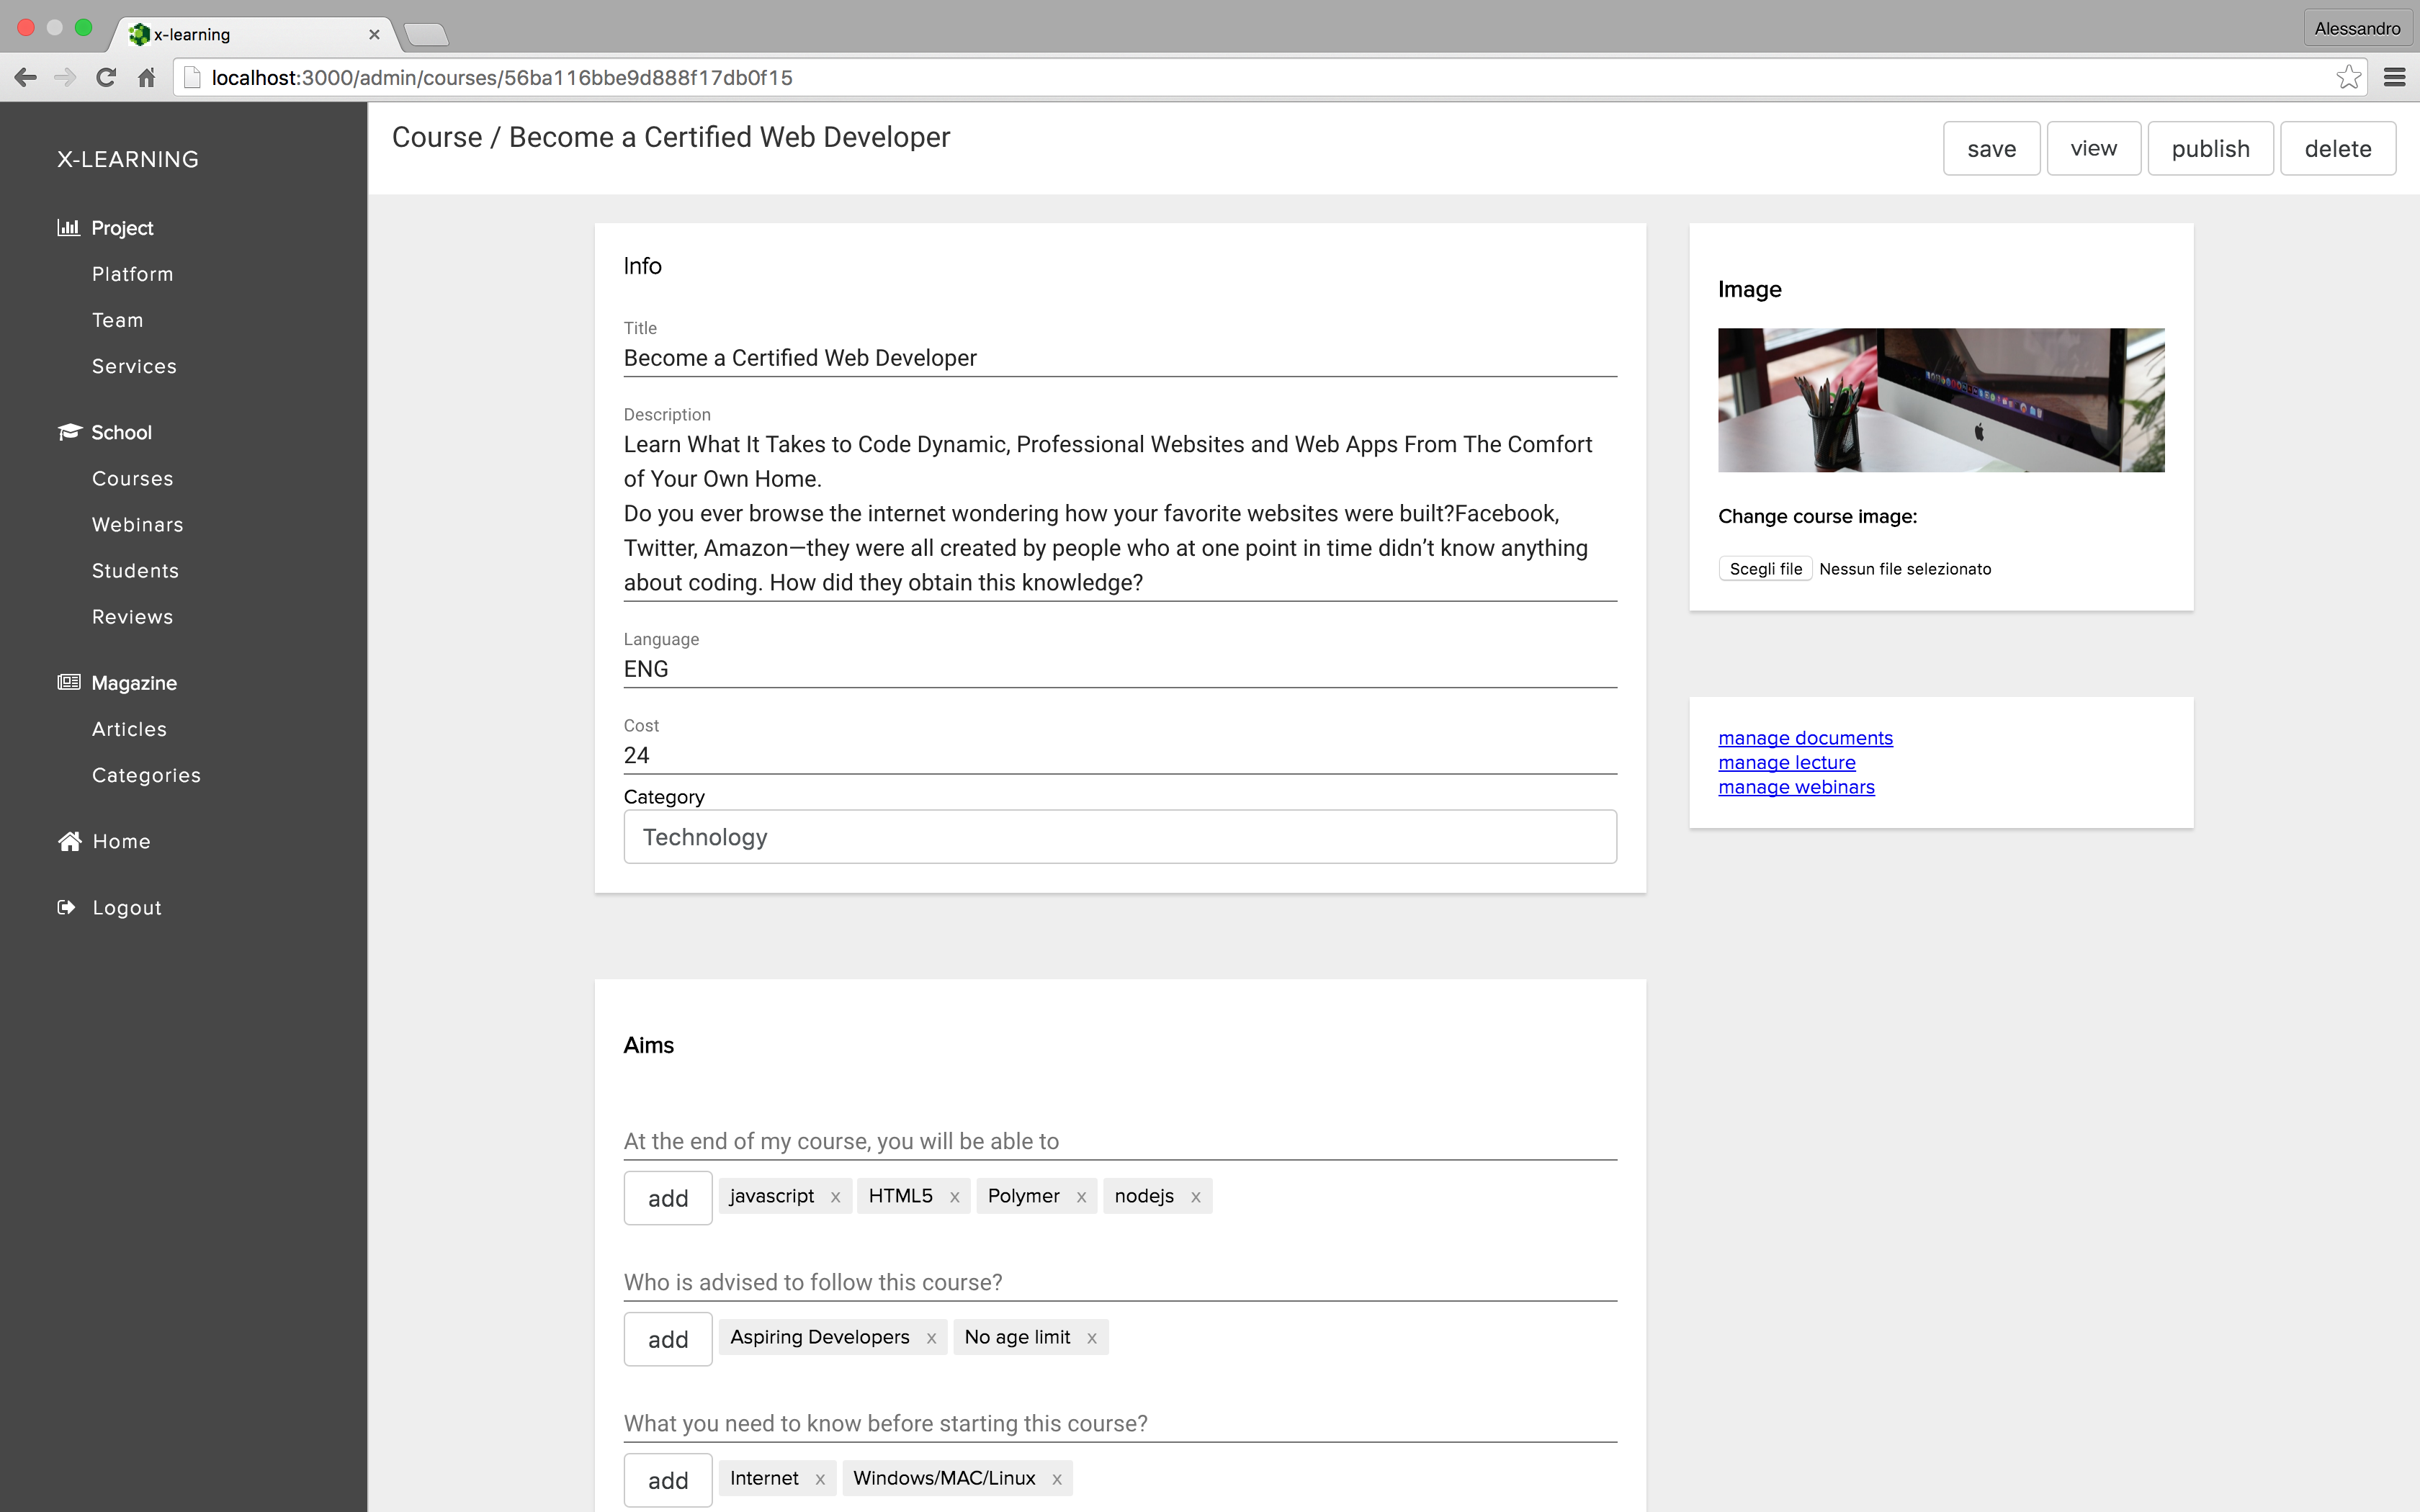
\includegraphics[width=1.0\linewidth]{images/chapter4/page-course-admin.png}\hfill
 \caption[Page Admin course action]{Page Admin course action}
 \label{fig:fourV}
\end{figure}

The image below shows course's edit page composed by the following Web components:

\begin{lstlisting}[language=html]
<part-course-actions course="{{course}}"></part-course-actions>
\end{lstlisting}
this component is used to represent buttons to perform the action in the course;

\begin{lstlisting}[language=html]
<part-course-aims course="{{course}}"></part-course-aims>
\end{lstlisting}
this component is used to insert the aims of the course;

\begin{lstlisting}[language=html]
<part-course-image course="{{course}}"></part-course-image>
\end{lstlisting}
this component is used to show and change the image of the course;

\begin{lstlisting}[language=html]
<part-course-info course="{{course}}"></part-course-info>
\end{lstlisting}
this element manages information based on a course such as the name and description;


Each component inside is made up, in turn, by other components. This can be seen, for example, in the part-course-info code.

\begin{lstlisting}[language=html]
<dom-module id="form-course-info">
  <template>
    <style include="style-form"></style>

    <form on-submit="on_submit">
      <div class="field">
        <paper-input label="Title" id="title" type="text" value="{{course.title}}"></paper-input>
        <paper-textarea label="Description" value="{{course.description}}"></paper-textarea>
      
        <paper-input label="Language" id="title" type="text" value="{{course.language}}"></paper-input>
        <paper-input label="Cost" id="title" type="number" value="{{course.cost}}"></paper-input>
      </div>
      <div class="field">
        <search-course-category course="{{course}}" on-try-save-categories="on_try_save_categories" on-try-delete-category="on_try_delete_category"></search-course-category>
      </div>
    </form>

  </template>
</dom-module>
\end{lstlisting}


% Also as you can see on the page is given the opportunity to manage the different components of the course:
% \begin{itemize}

% \item \textbf{Image section}\par
% \begin{itemize}
%   \item add the image of the course
%   \item change the image of the course
% \end{itemize}

% \item \textbf{Aims section} permette di inserire:

% \begin{itemize}
%   \item At the end of my course, students will be able to
%   \item Who is advised to follow this course, and who is not ?
%   \item What students need to know or do before you start your course ?
% \end{itemize}

% \item \textbf{Lectures section}\par 
% \begin{itemize}
%   \item manage the lessons of the course and so change and elimination
%   \item link to the page for creating a new lesson that lets you enter information such as title description and upload the video  
% \end{itemize}


% \item \textbf{Webinar section}\par
% \begin{itemize}
%   \item manage the webinar of the course and so change and elimination
%   \item link to the page for creating a new lesson that lets you enter information such as title description and set the date
% \end{itemize}


% \item \textbf{Document}\par
% \begin{itemize}
%   \item add documents to the course
%   \item remove documents from the course
% \end{itemize}

% \end{itemize}

\newpage
\subsection {Pages on Admin and Client side}
\label{subsec:pages}
The same approach just illustrated is reused to create the entire platform.
Without going into detail, a few of the main pages that compose the thesis project will be shown.

\subsubsection {Pages on Admin side}
\label{subsec:Admin_side}

The admin side is the part of the platform that enables the Manager to manage the courses and all its sub-components such as lectures, webinars, educational material.

The main page is presented as following:
\\

\begin{minipage}{\linewidth}
    \centering
    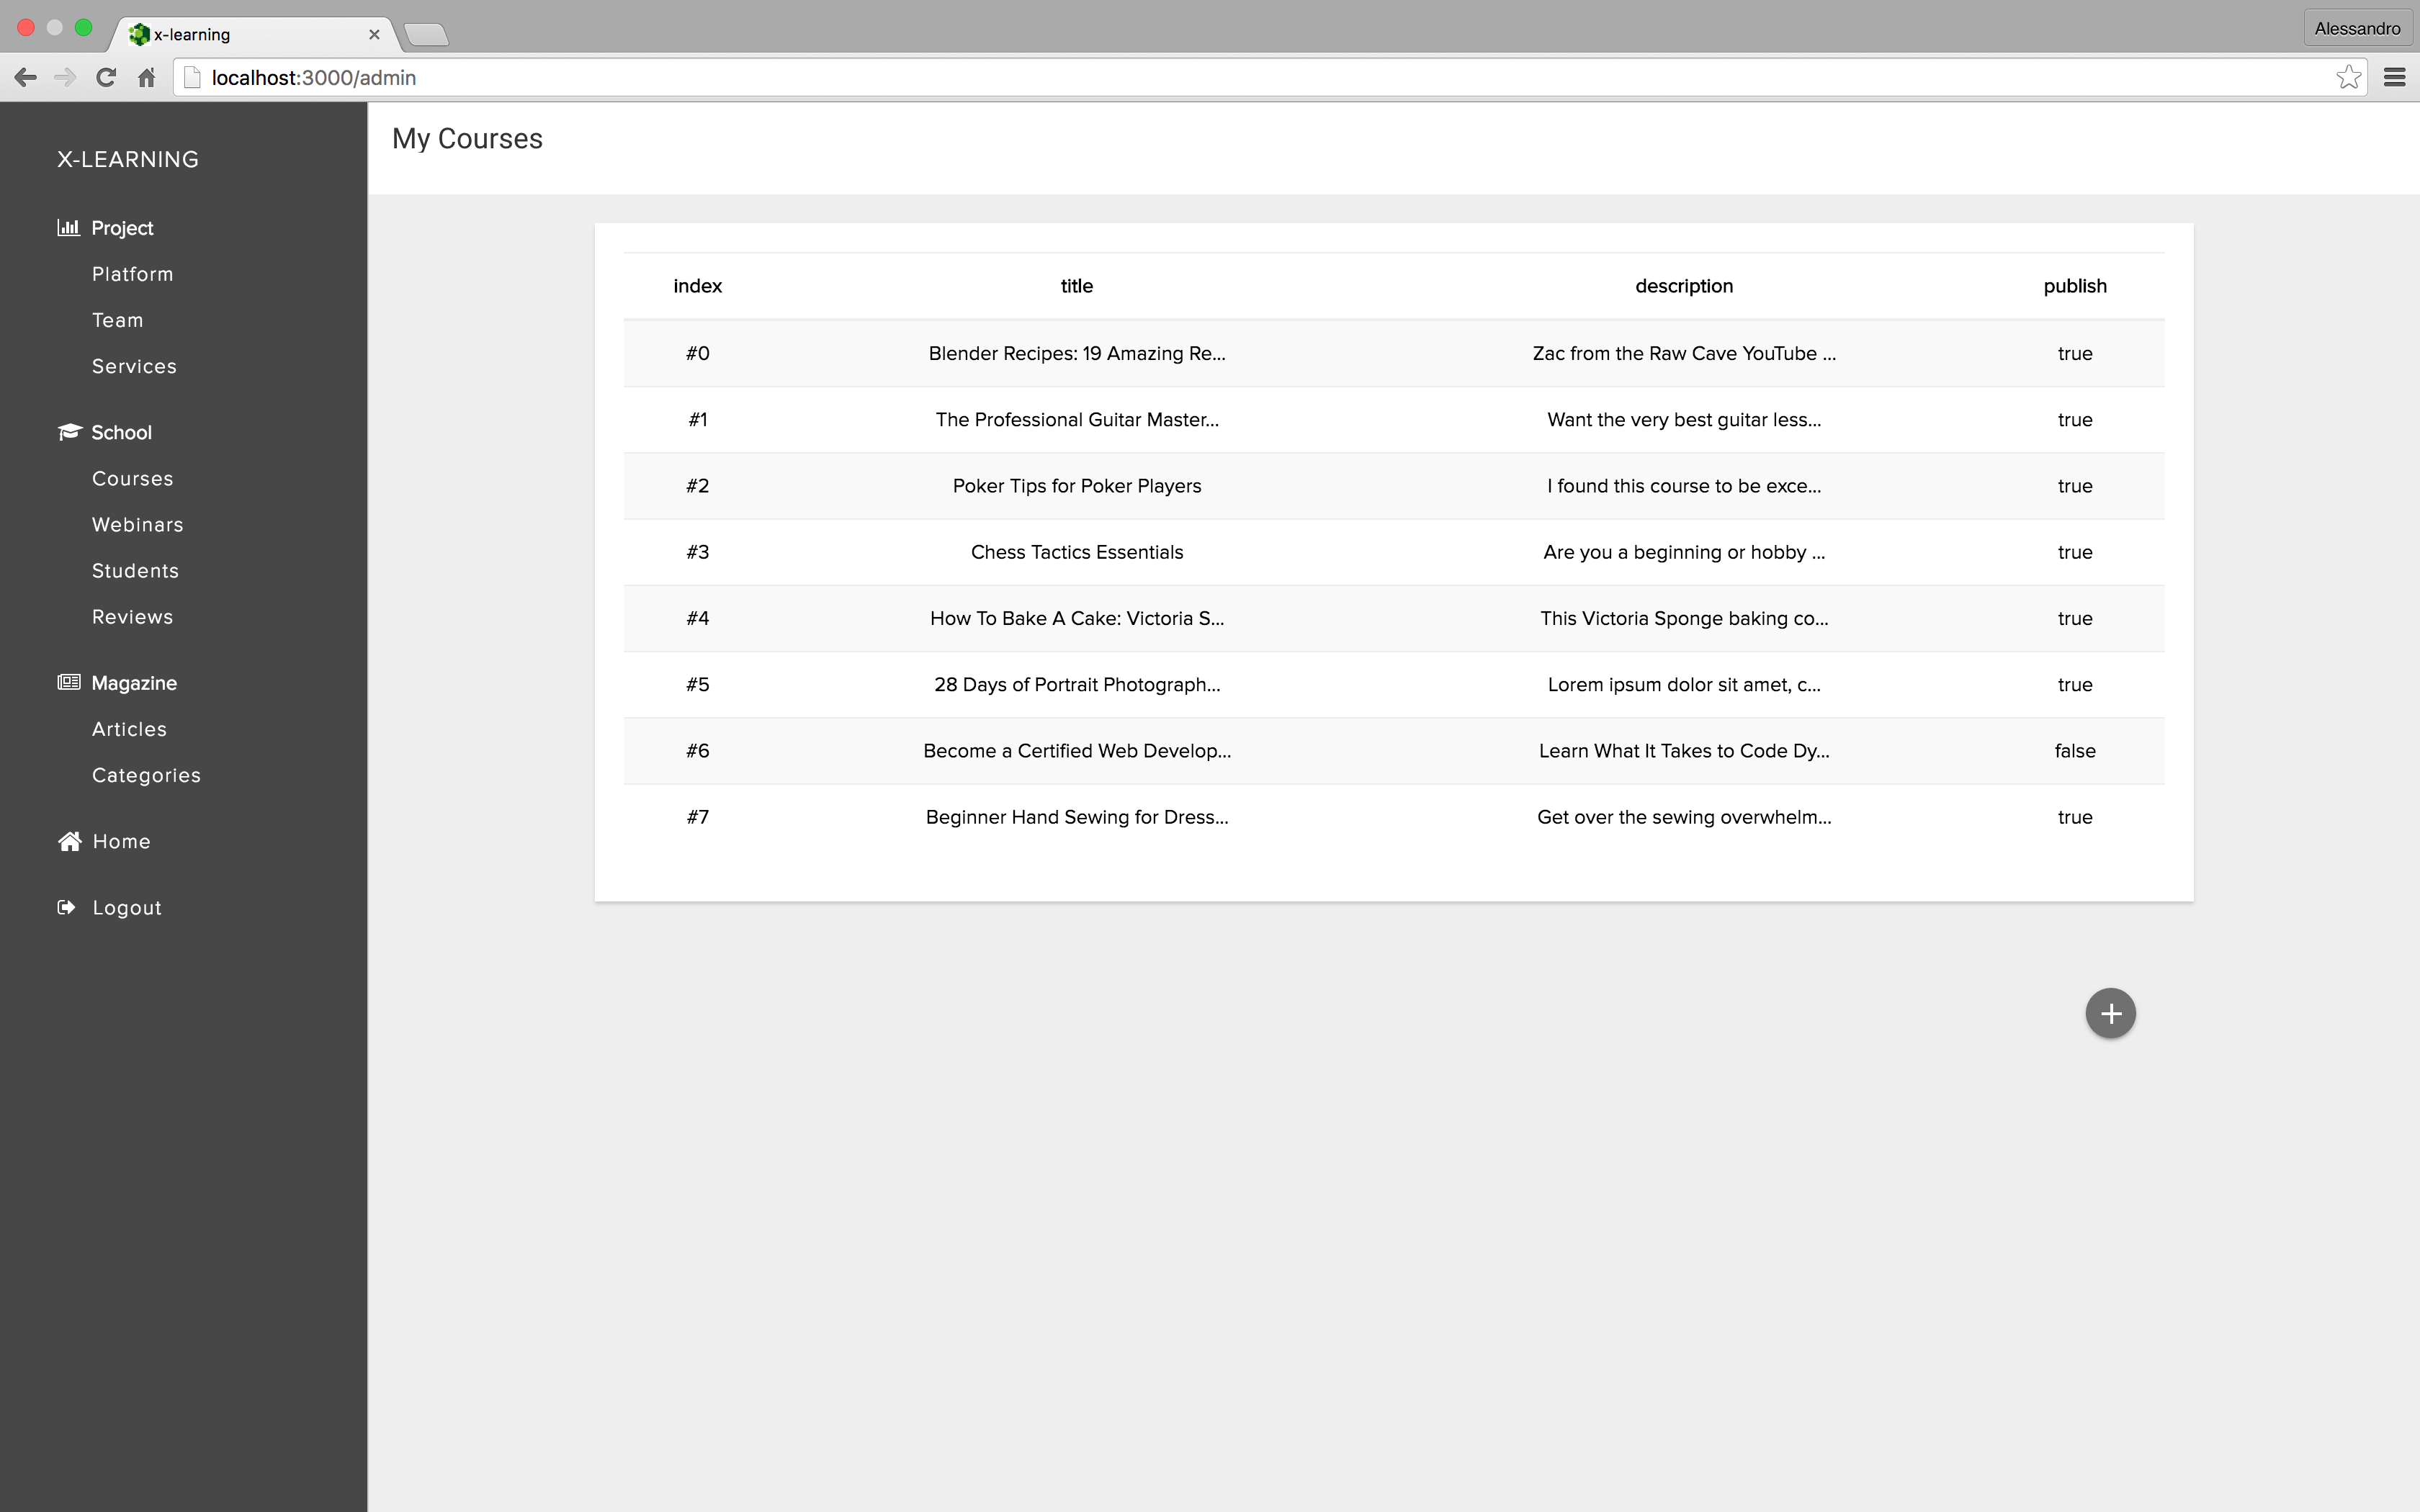
\includegraphics[width=0.9\linewidth]{images/chapter4/page-admin.png}
    \captionof{figure}[Page Home Admin]{Page Home Admin}
\end{minipage}
\\

The main pages that compose the admin side are:

\begin{itemize}
\item \textbf{Page Course} The following image represents the course's page where the teacher can manage the creation and modification of all the course information.\par

\begin{minipage}{\linewidth}
    \centering
    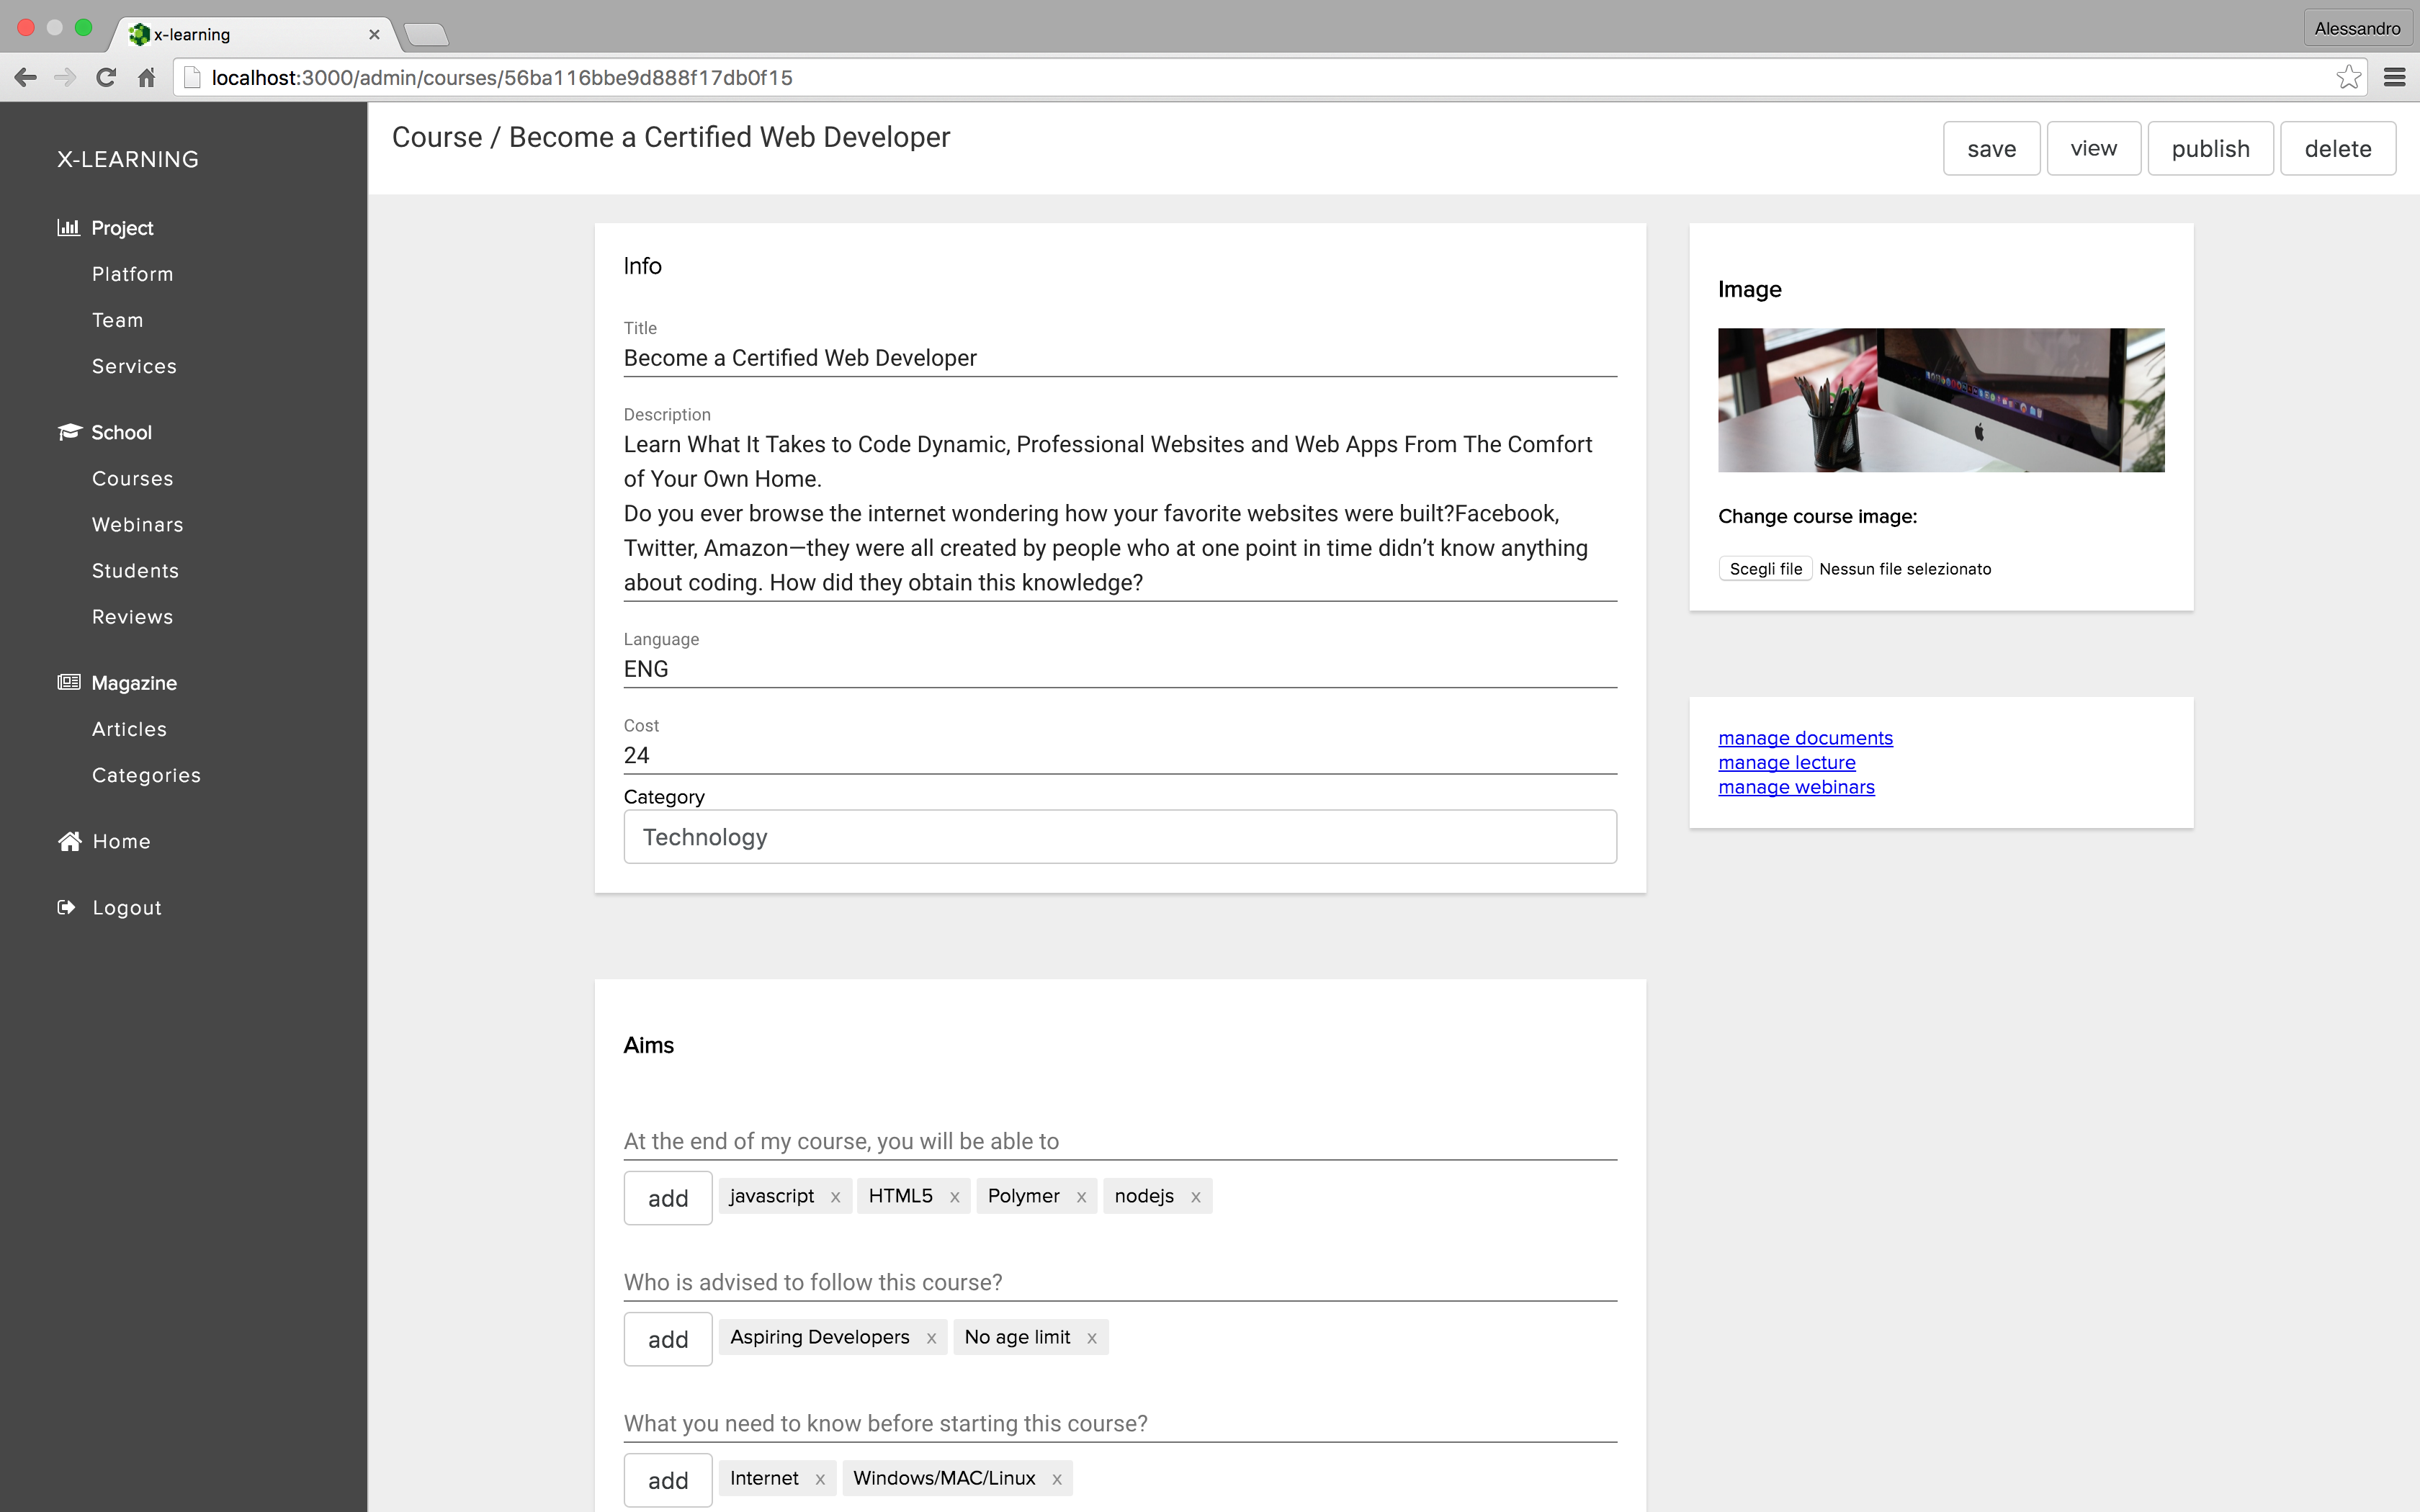
\includegraphics[width=0.9\linewidth]{images/chapter4/page-course-admin.png}
    \captionof{figure}[Page Course Admin]{Page Course Admin}
\end{minipage}

\item \textbf{Page Lecture} The following image represents the lecture's page where the teacher can manage the creation and modification of the single lecture information and insert/change the video.
\\
\par

\begin{minipage}{\linewidth}
    \centering
    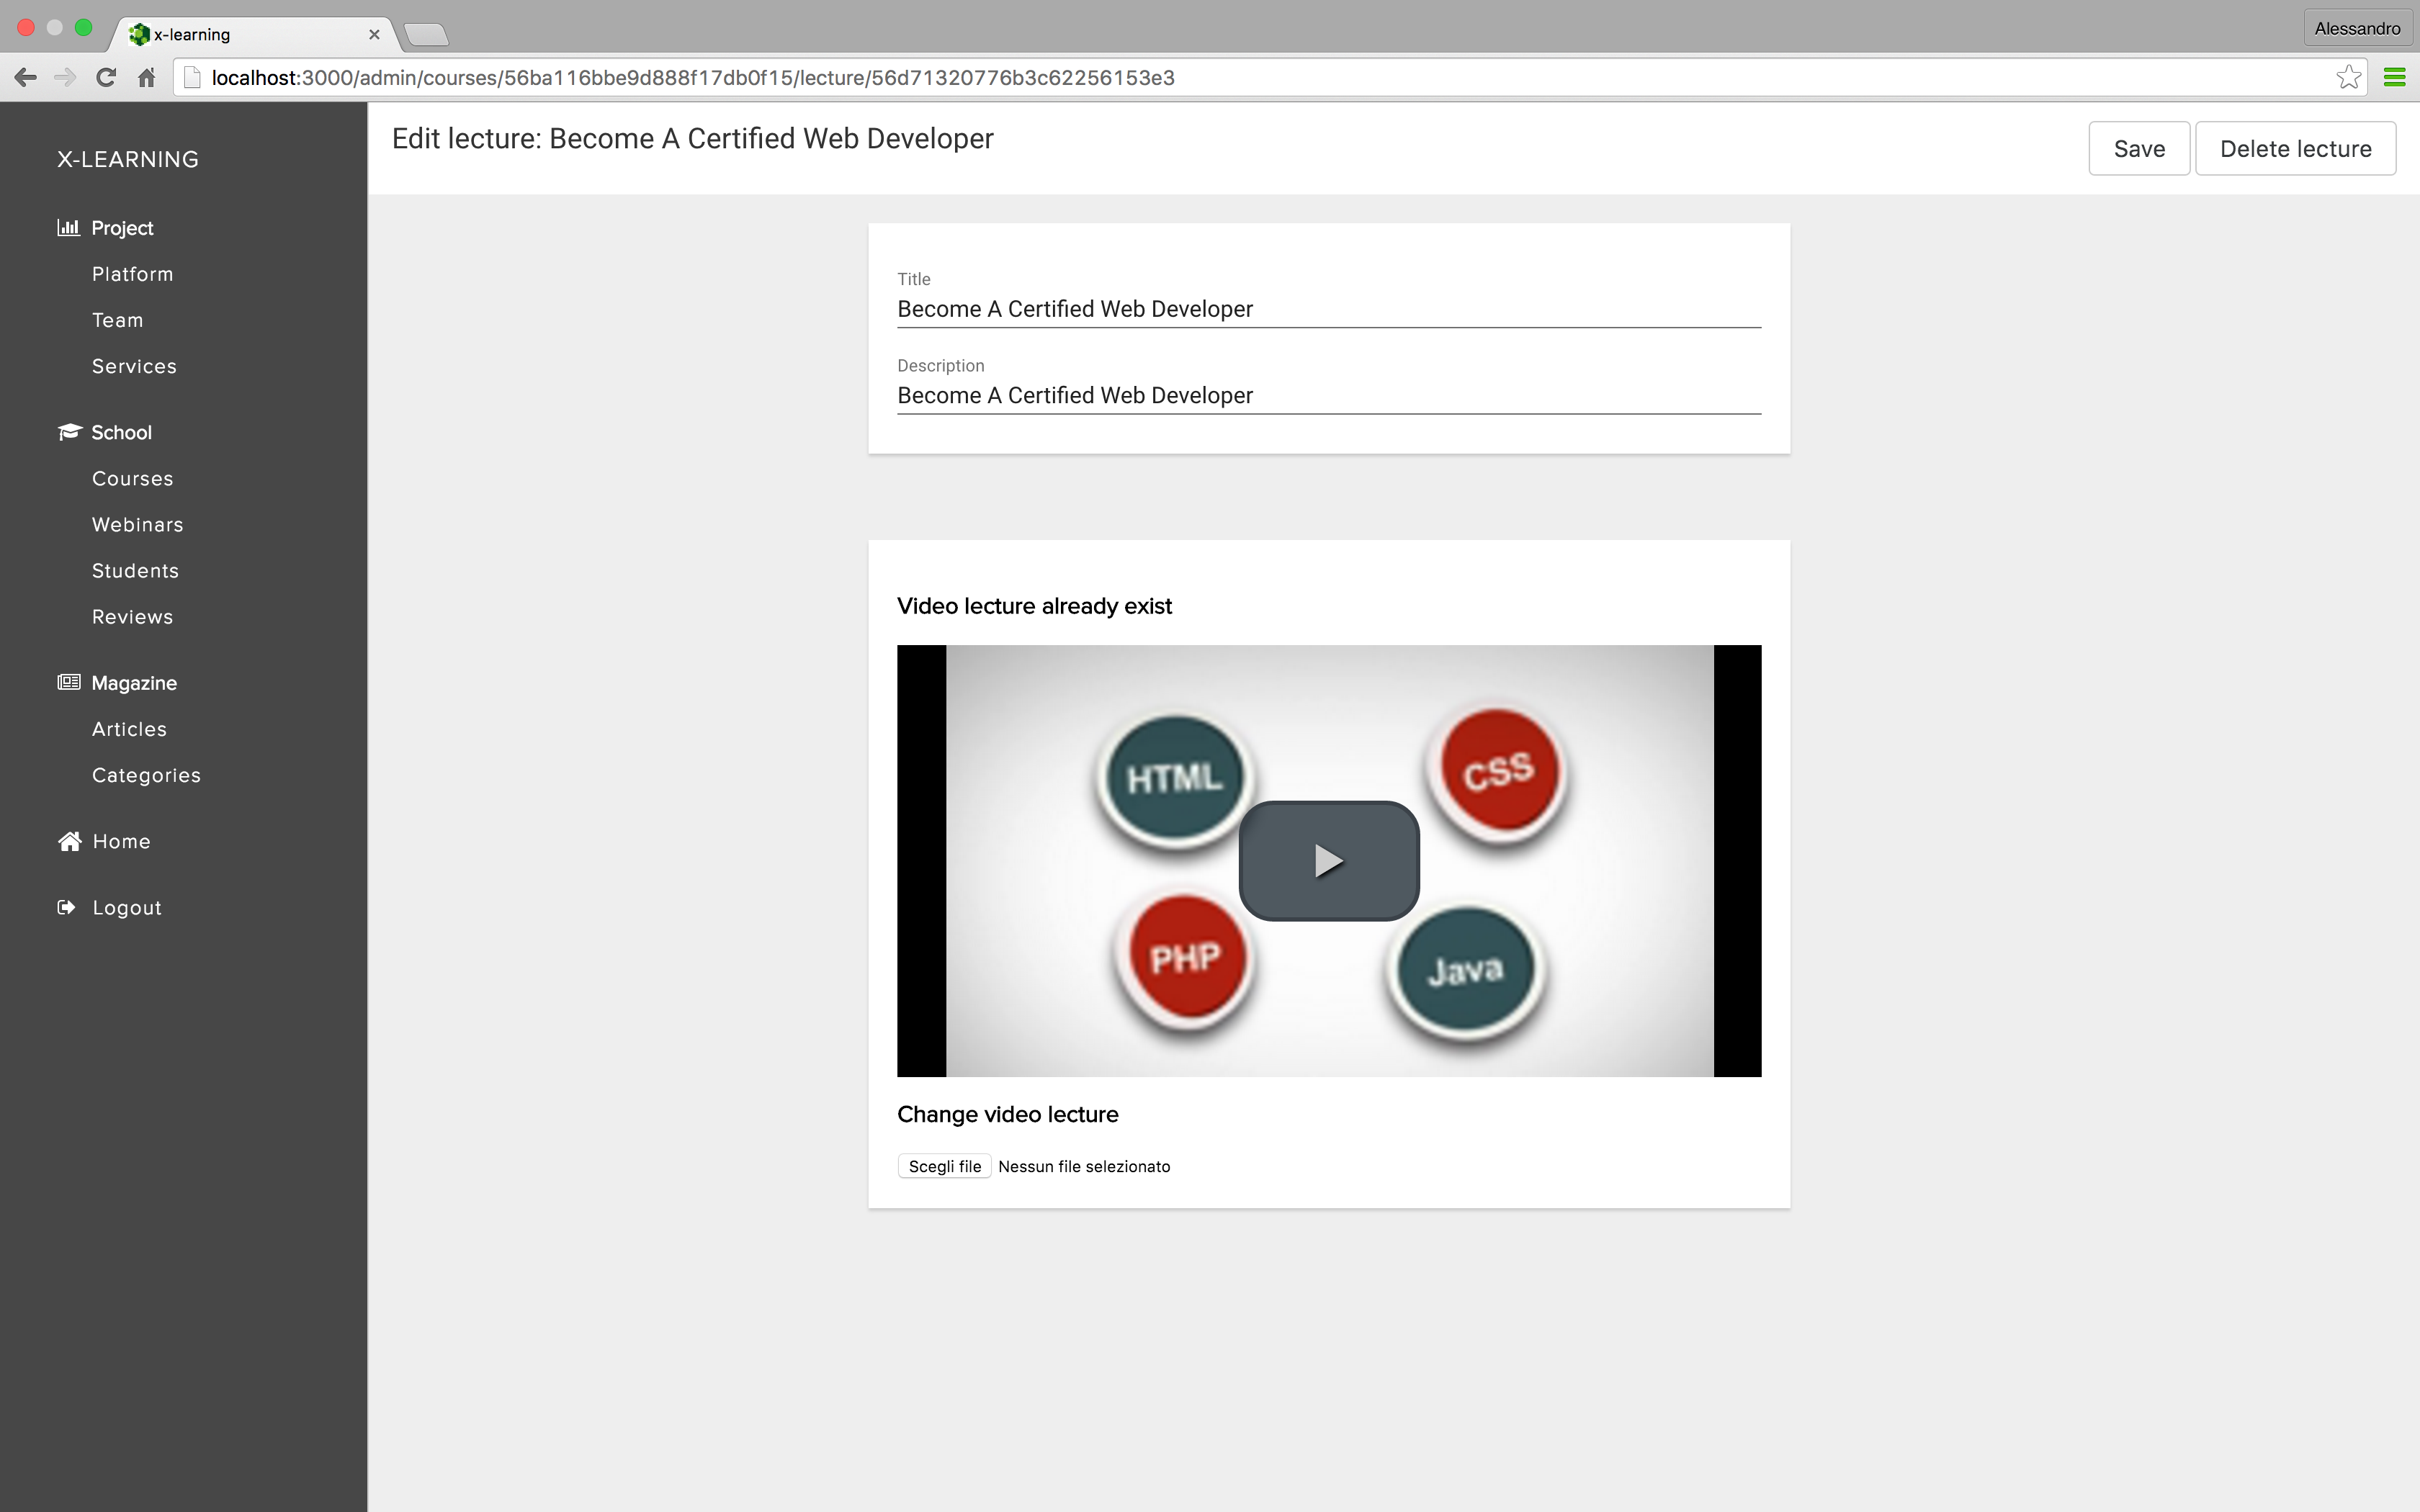
\includegraphics[width=0.9\linewidth]{images/chapter4/page-lecture-admin.png}
    \captionof{figure}[Page Lecture Admin]{Page Lecture Admin}
\end{minipage}

\item \textbf{Page Webinar} The following image represents the webinar's page where the teacher can manage the creation and modification of the single webinar information.
\par

\begin{minipage}{\linewidth}
    \centering
    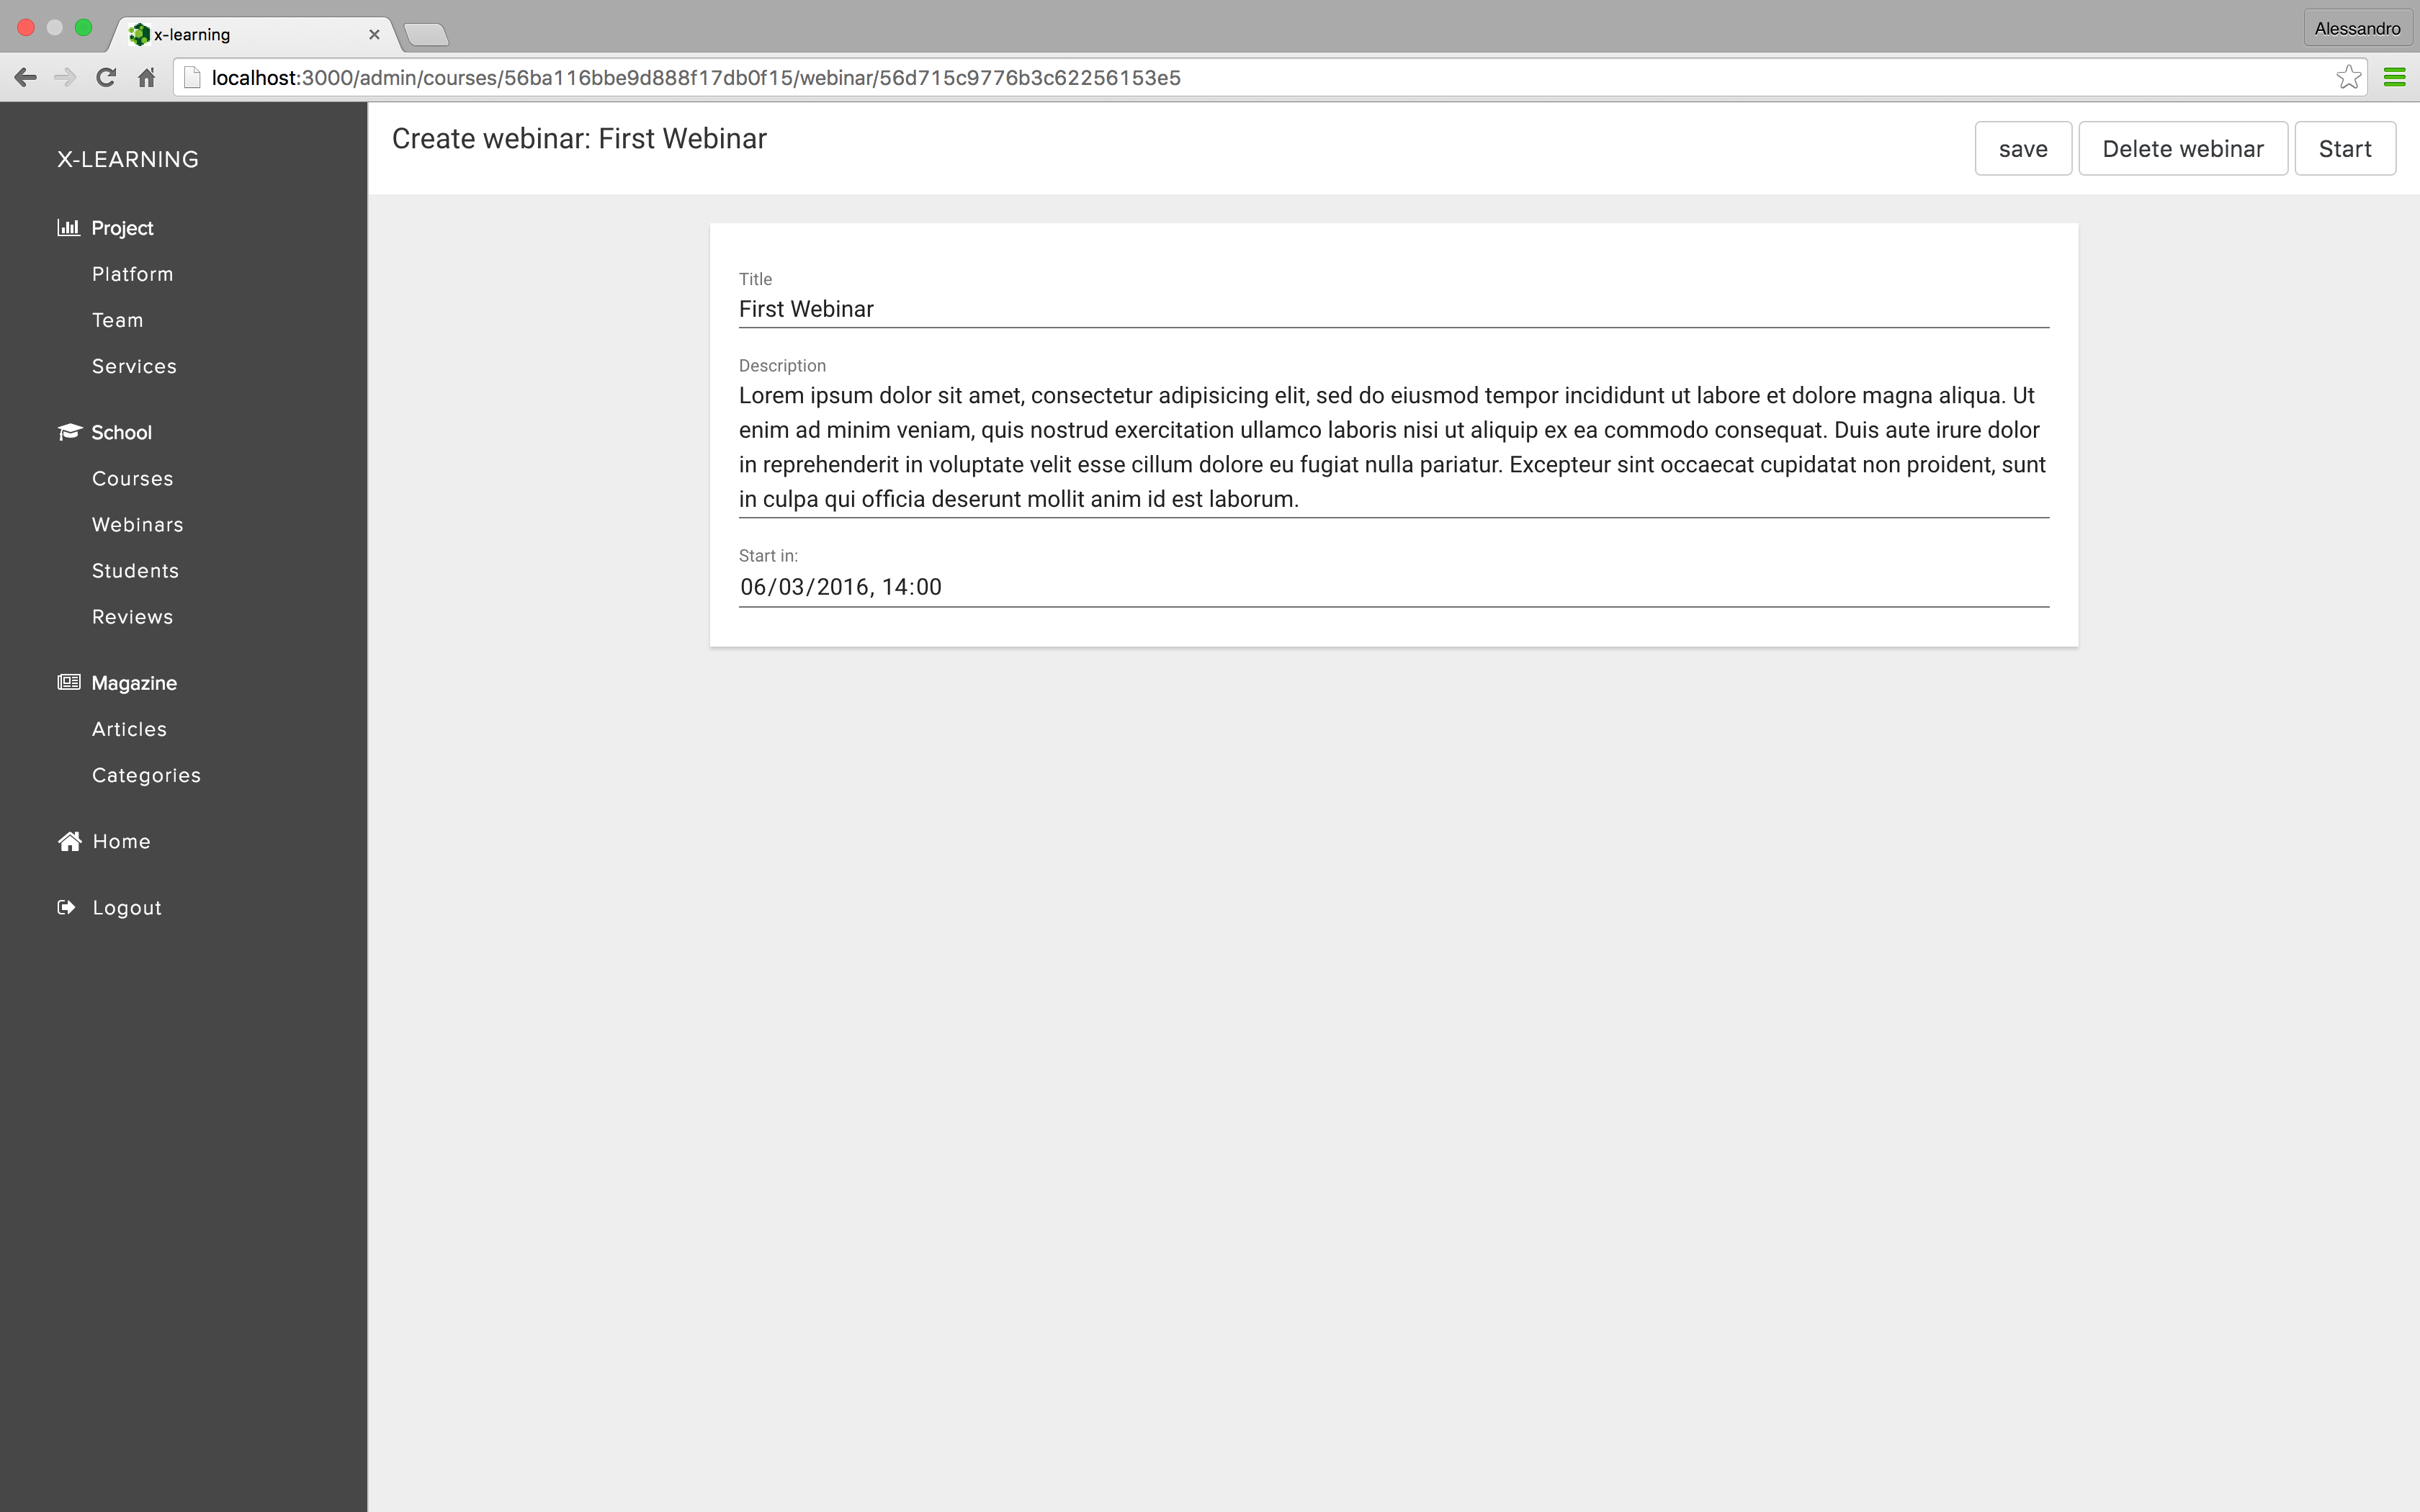
\includegraphics[width=0.9\linewidth]{images/chapter4/page-webinar-admin.png}
    \captionof{figure}[Page Webinar Admin]{Page Webinar Admin}
\end{minipage}

\item \textbf{Page Team} The following image represents the page in which the administrator can manage the teacher staff that can collaborate with the platform.
\\
\par

\begin{minipage}{\linewidth}
    \centering
    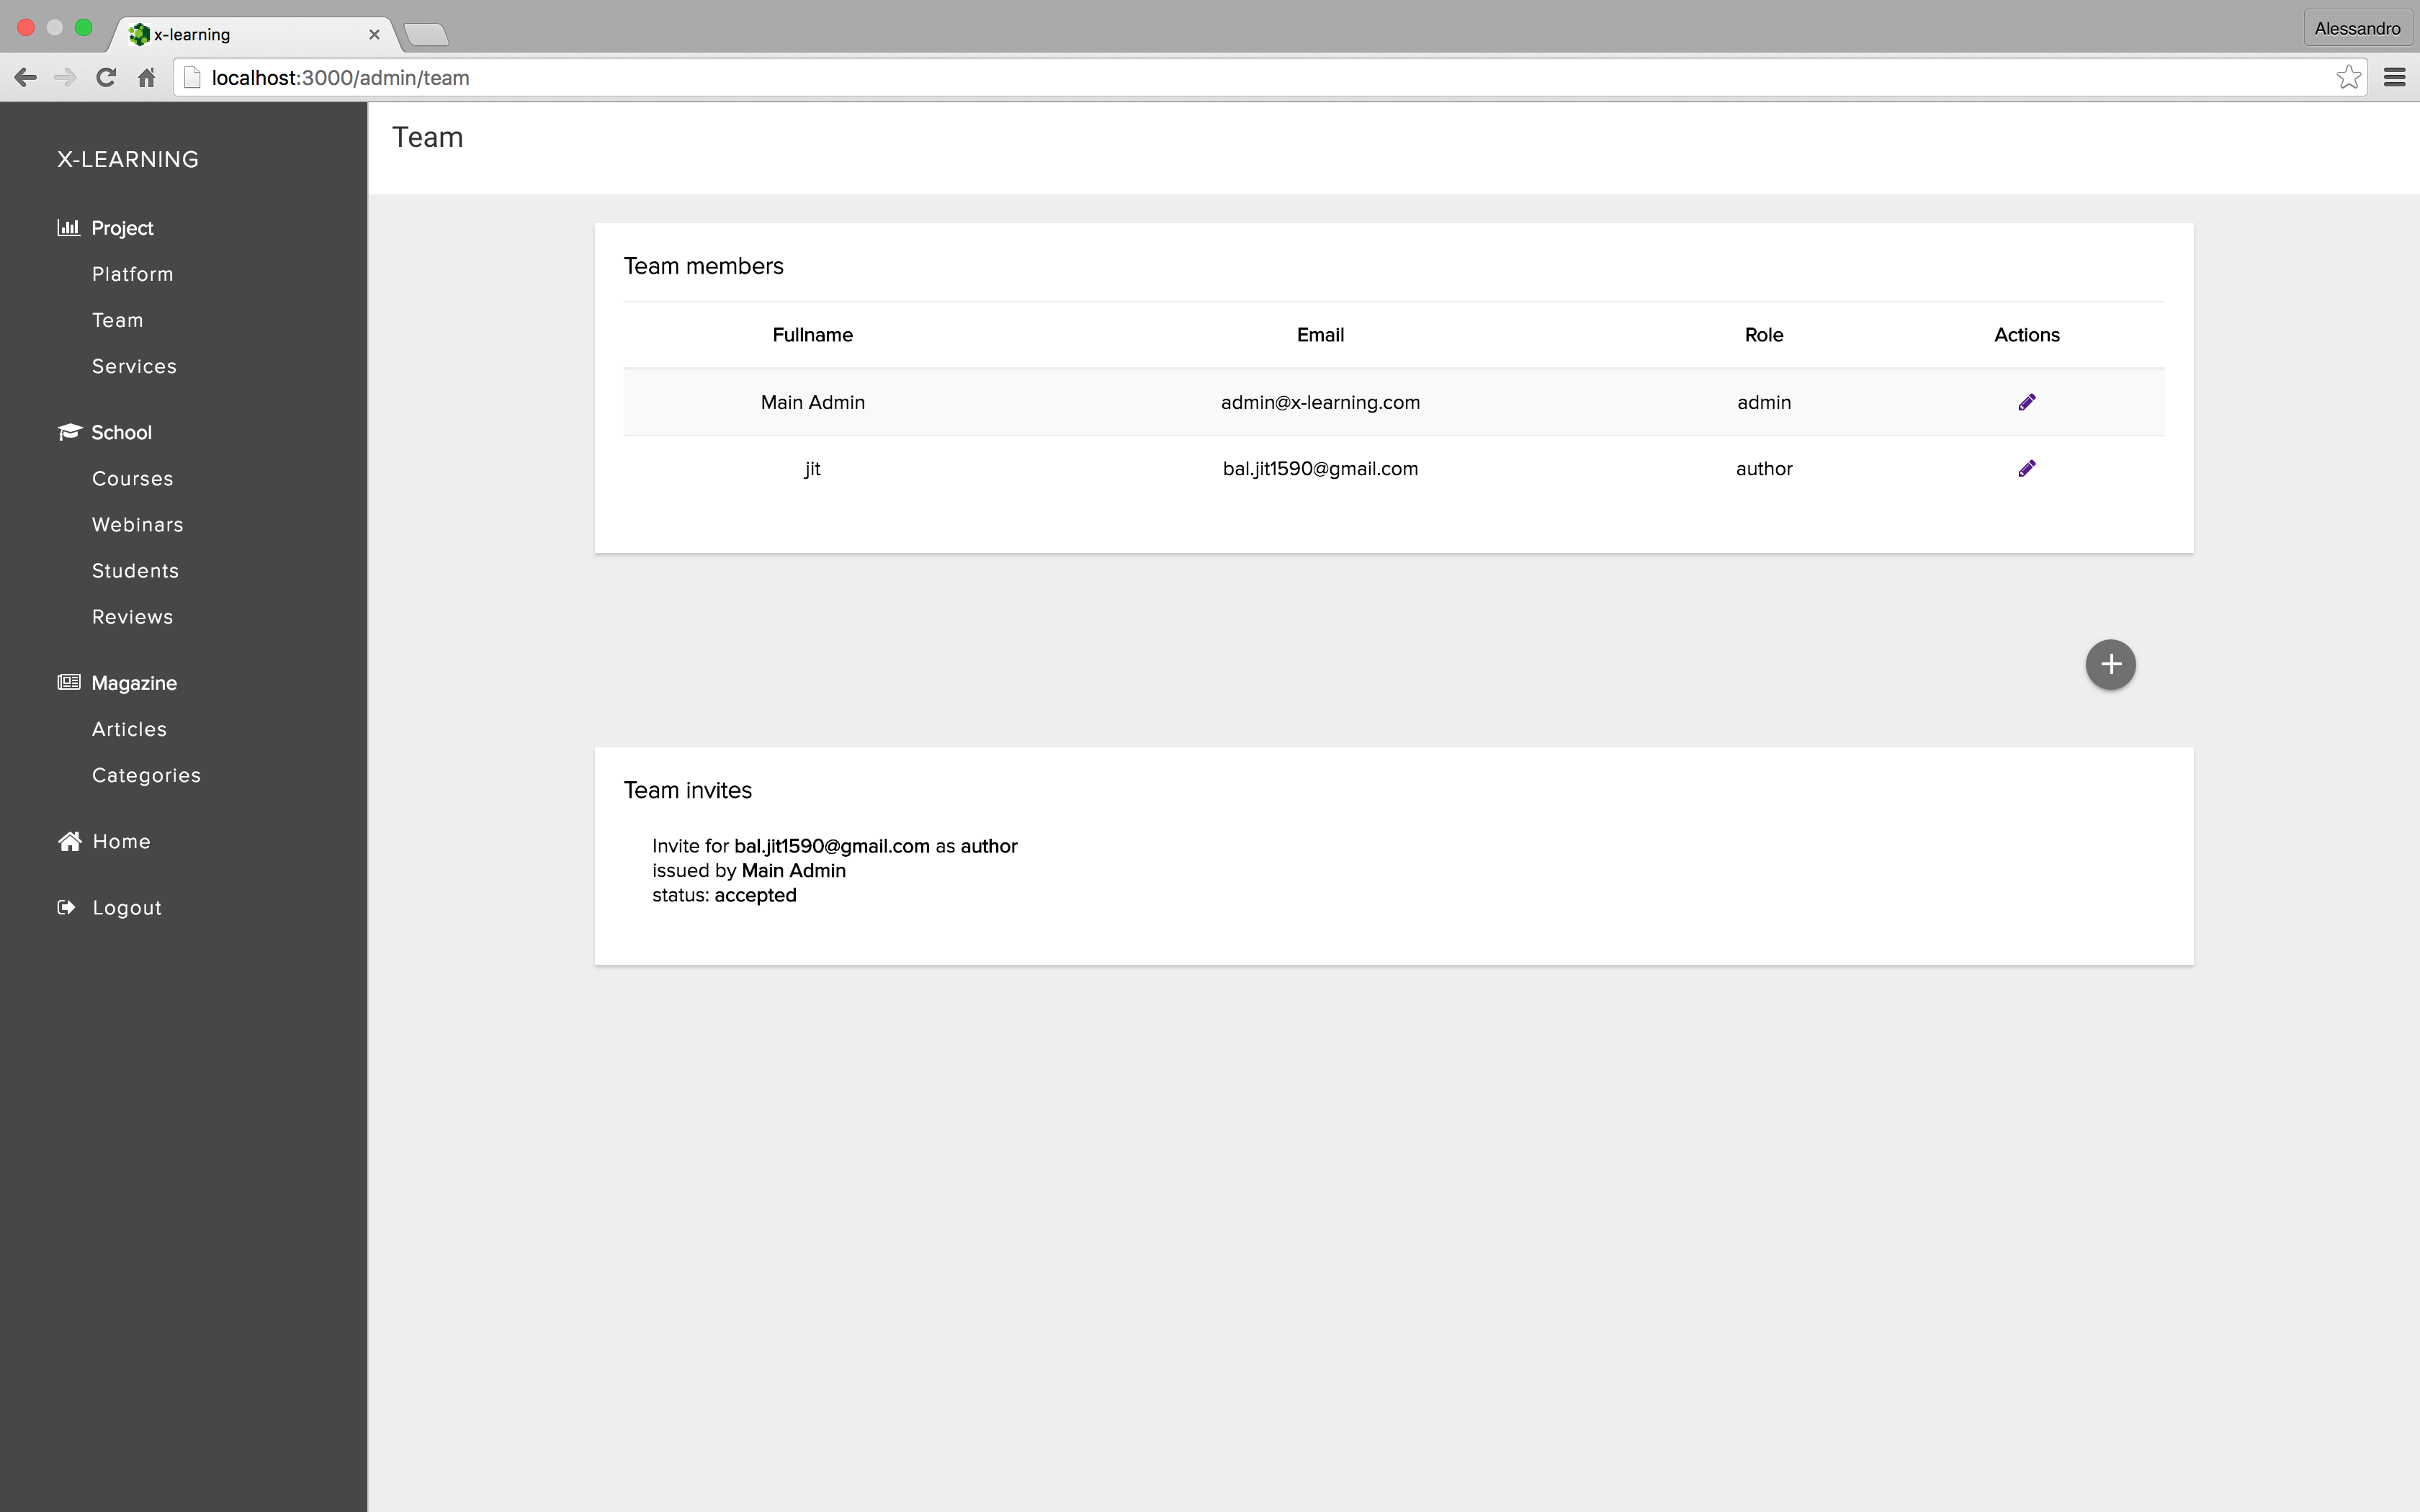
\includegraphics[width=0.9\linewidth]{images/chapter4/page-team-admin.png}
    \captionof{figure}[Page Team]{Page Team}
\end{minipage}

\item \textbf{Page Services} The following image represents the page in which the administrator can manage the insertion of various service codes utilized in the platform.
\\
\par

\begin{minipage}{\linewidth}
    \centering
    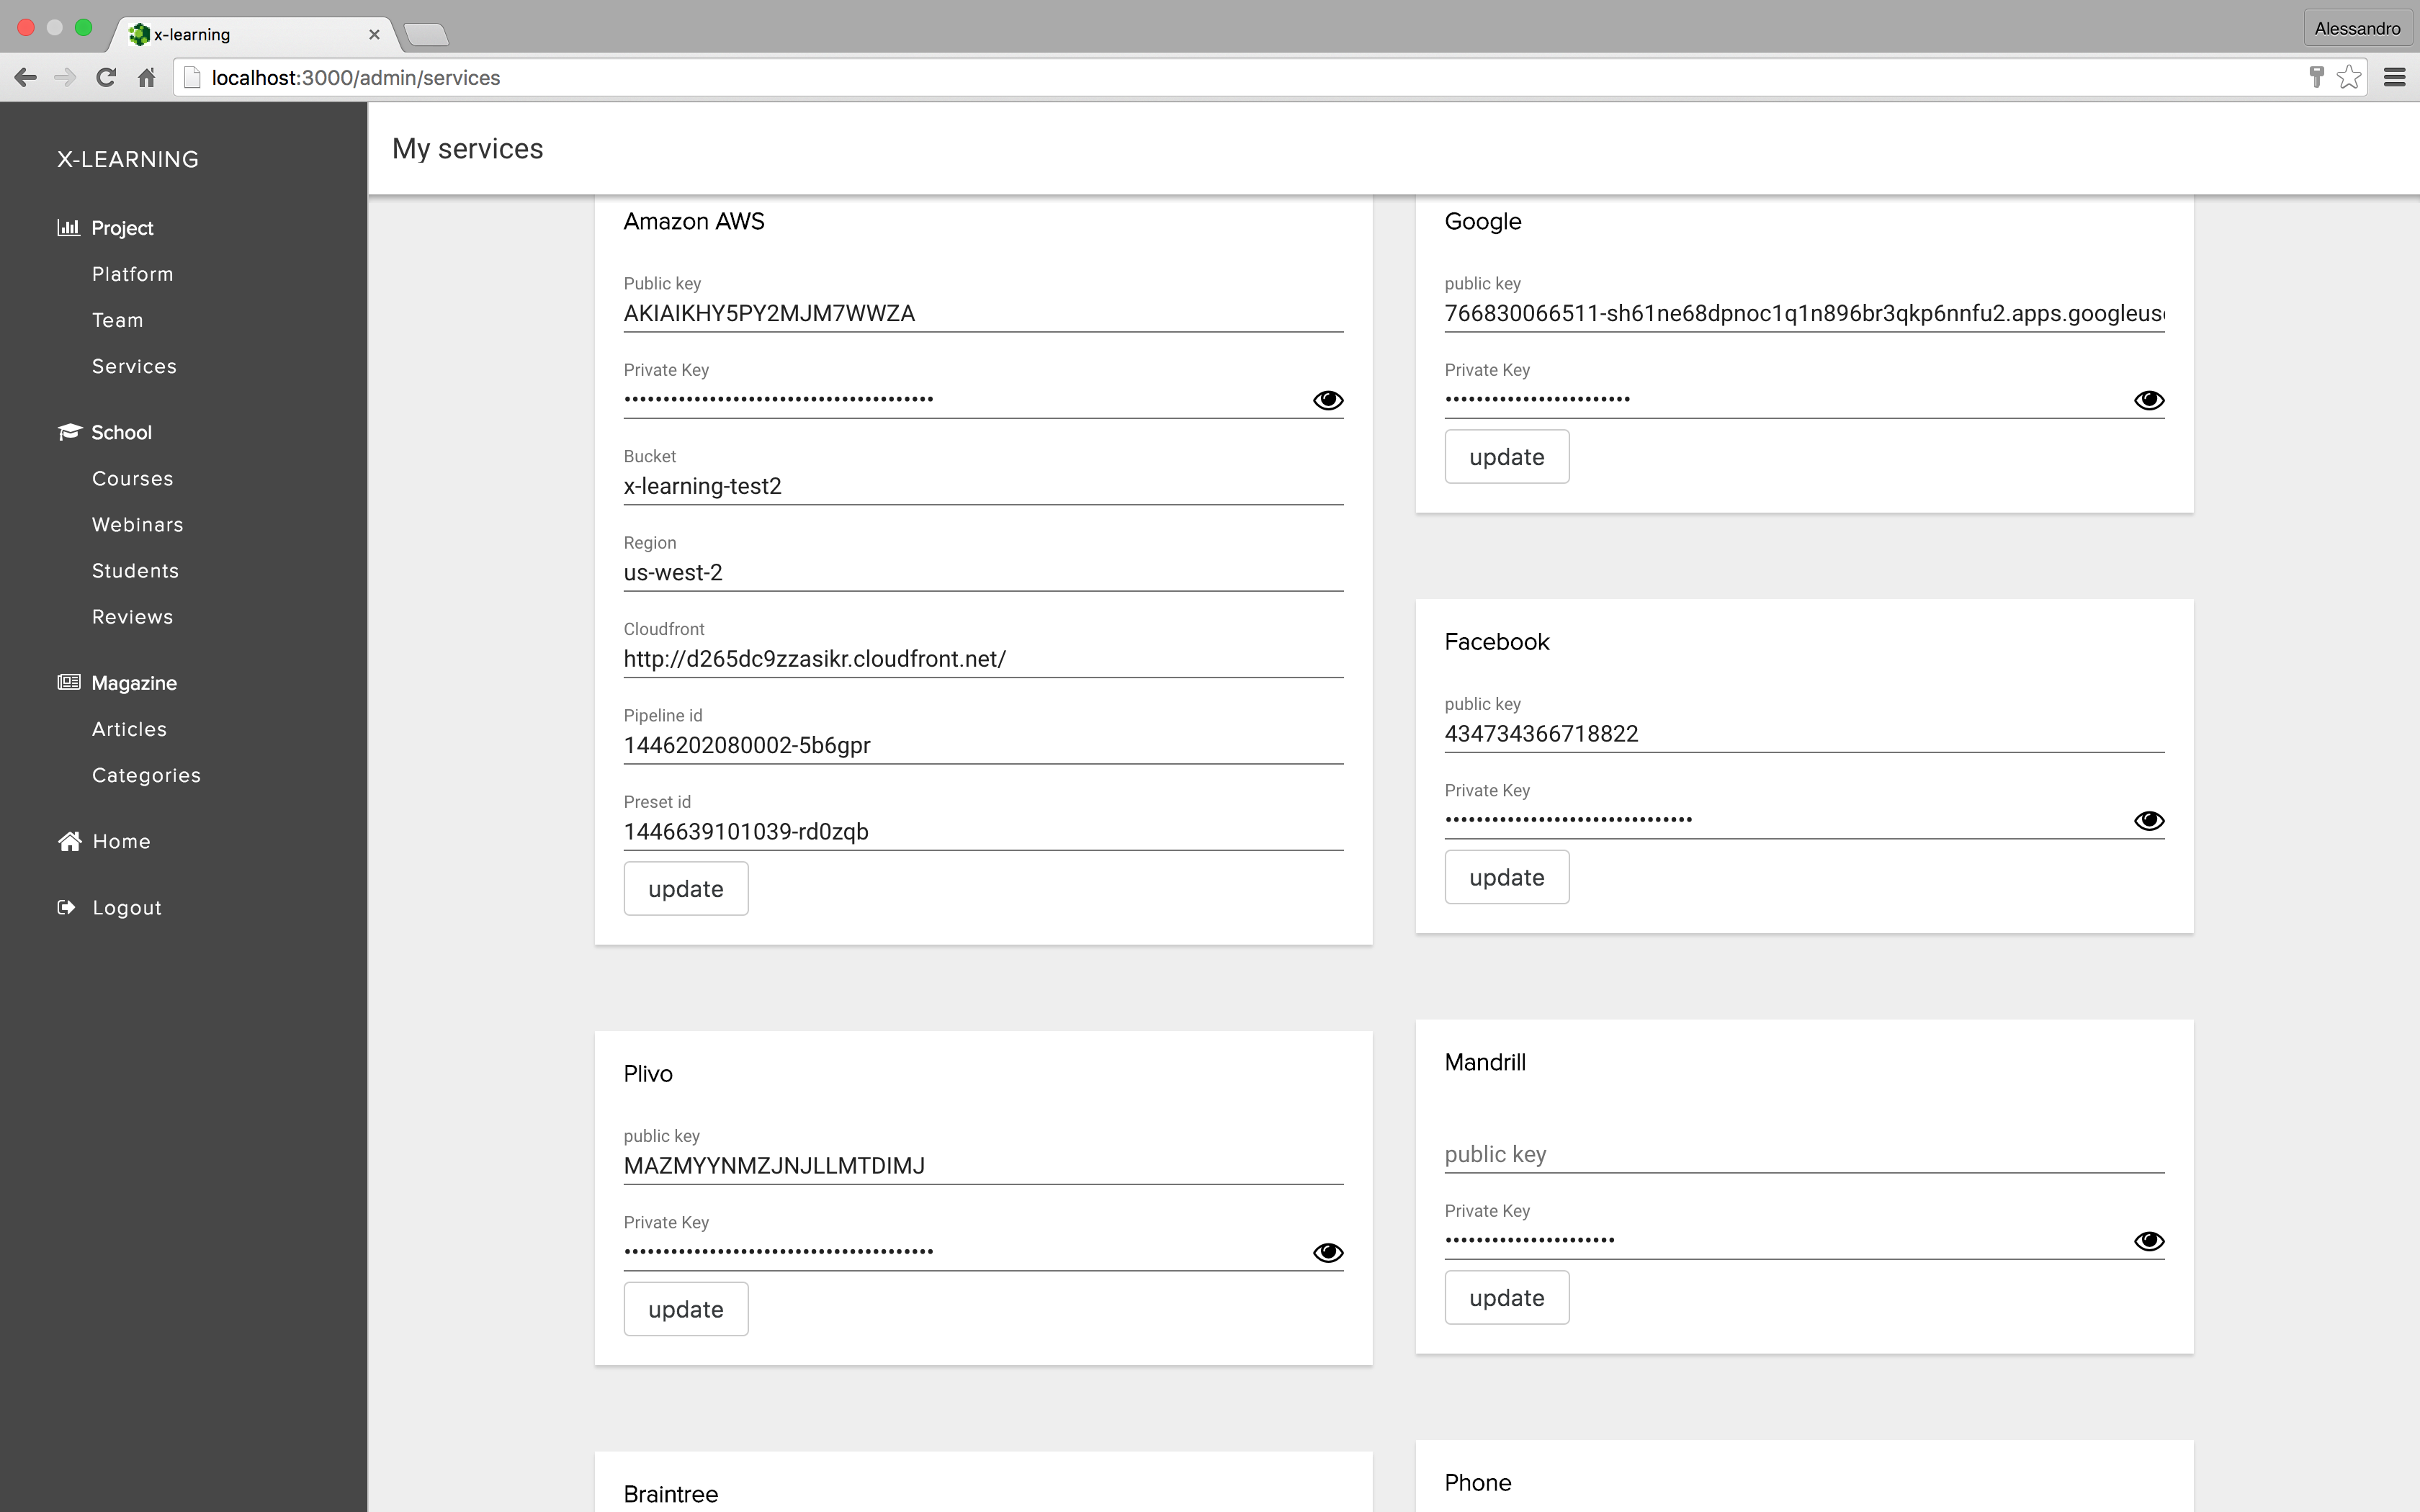
\includegraphics[width=0.9\linewidth]{images/chapter4/page-services-admin.png}
    \captionof{figure}[Page Services]{Page Services}
\end{minipage}

\end{itemize}


\subsubsection {Client side}
\label{subsec:Client_side}
The client side is the part of the platform that allows users to view courses and then attend lectures, webinars and access educational materials.

The main pages that compose the client side are:

\begin{itemize}

\item \textbf{Page Home} The following image represents the Home Page where the student can search for a specific course, see those that are available and possibly filter them by category.\par

\begin{minipage}{\linewidth}
    \centering
    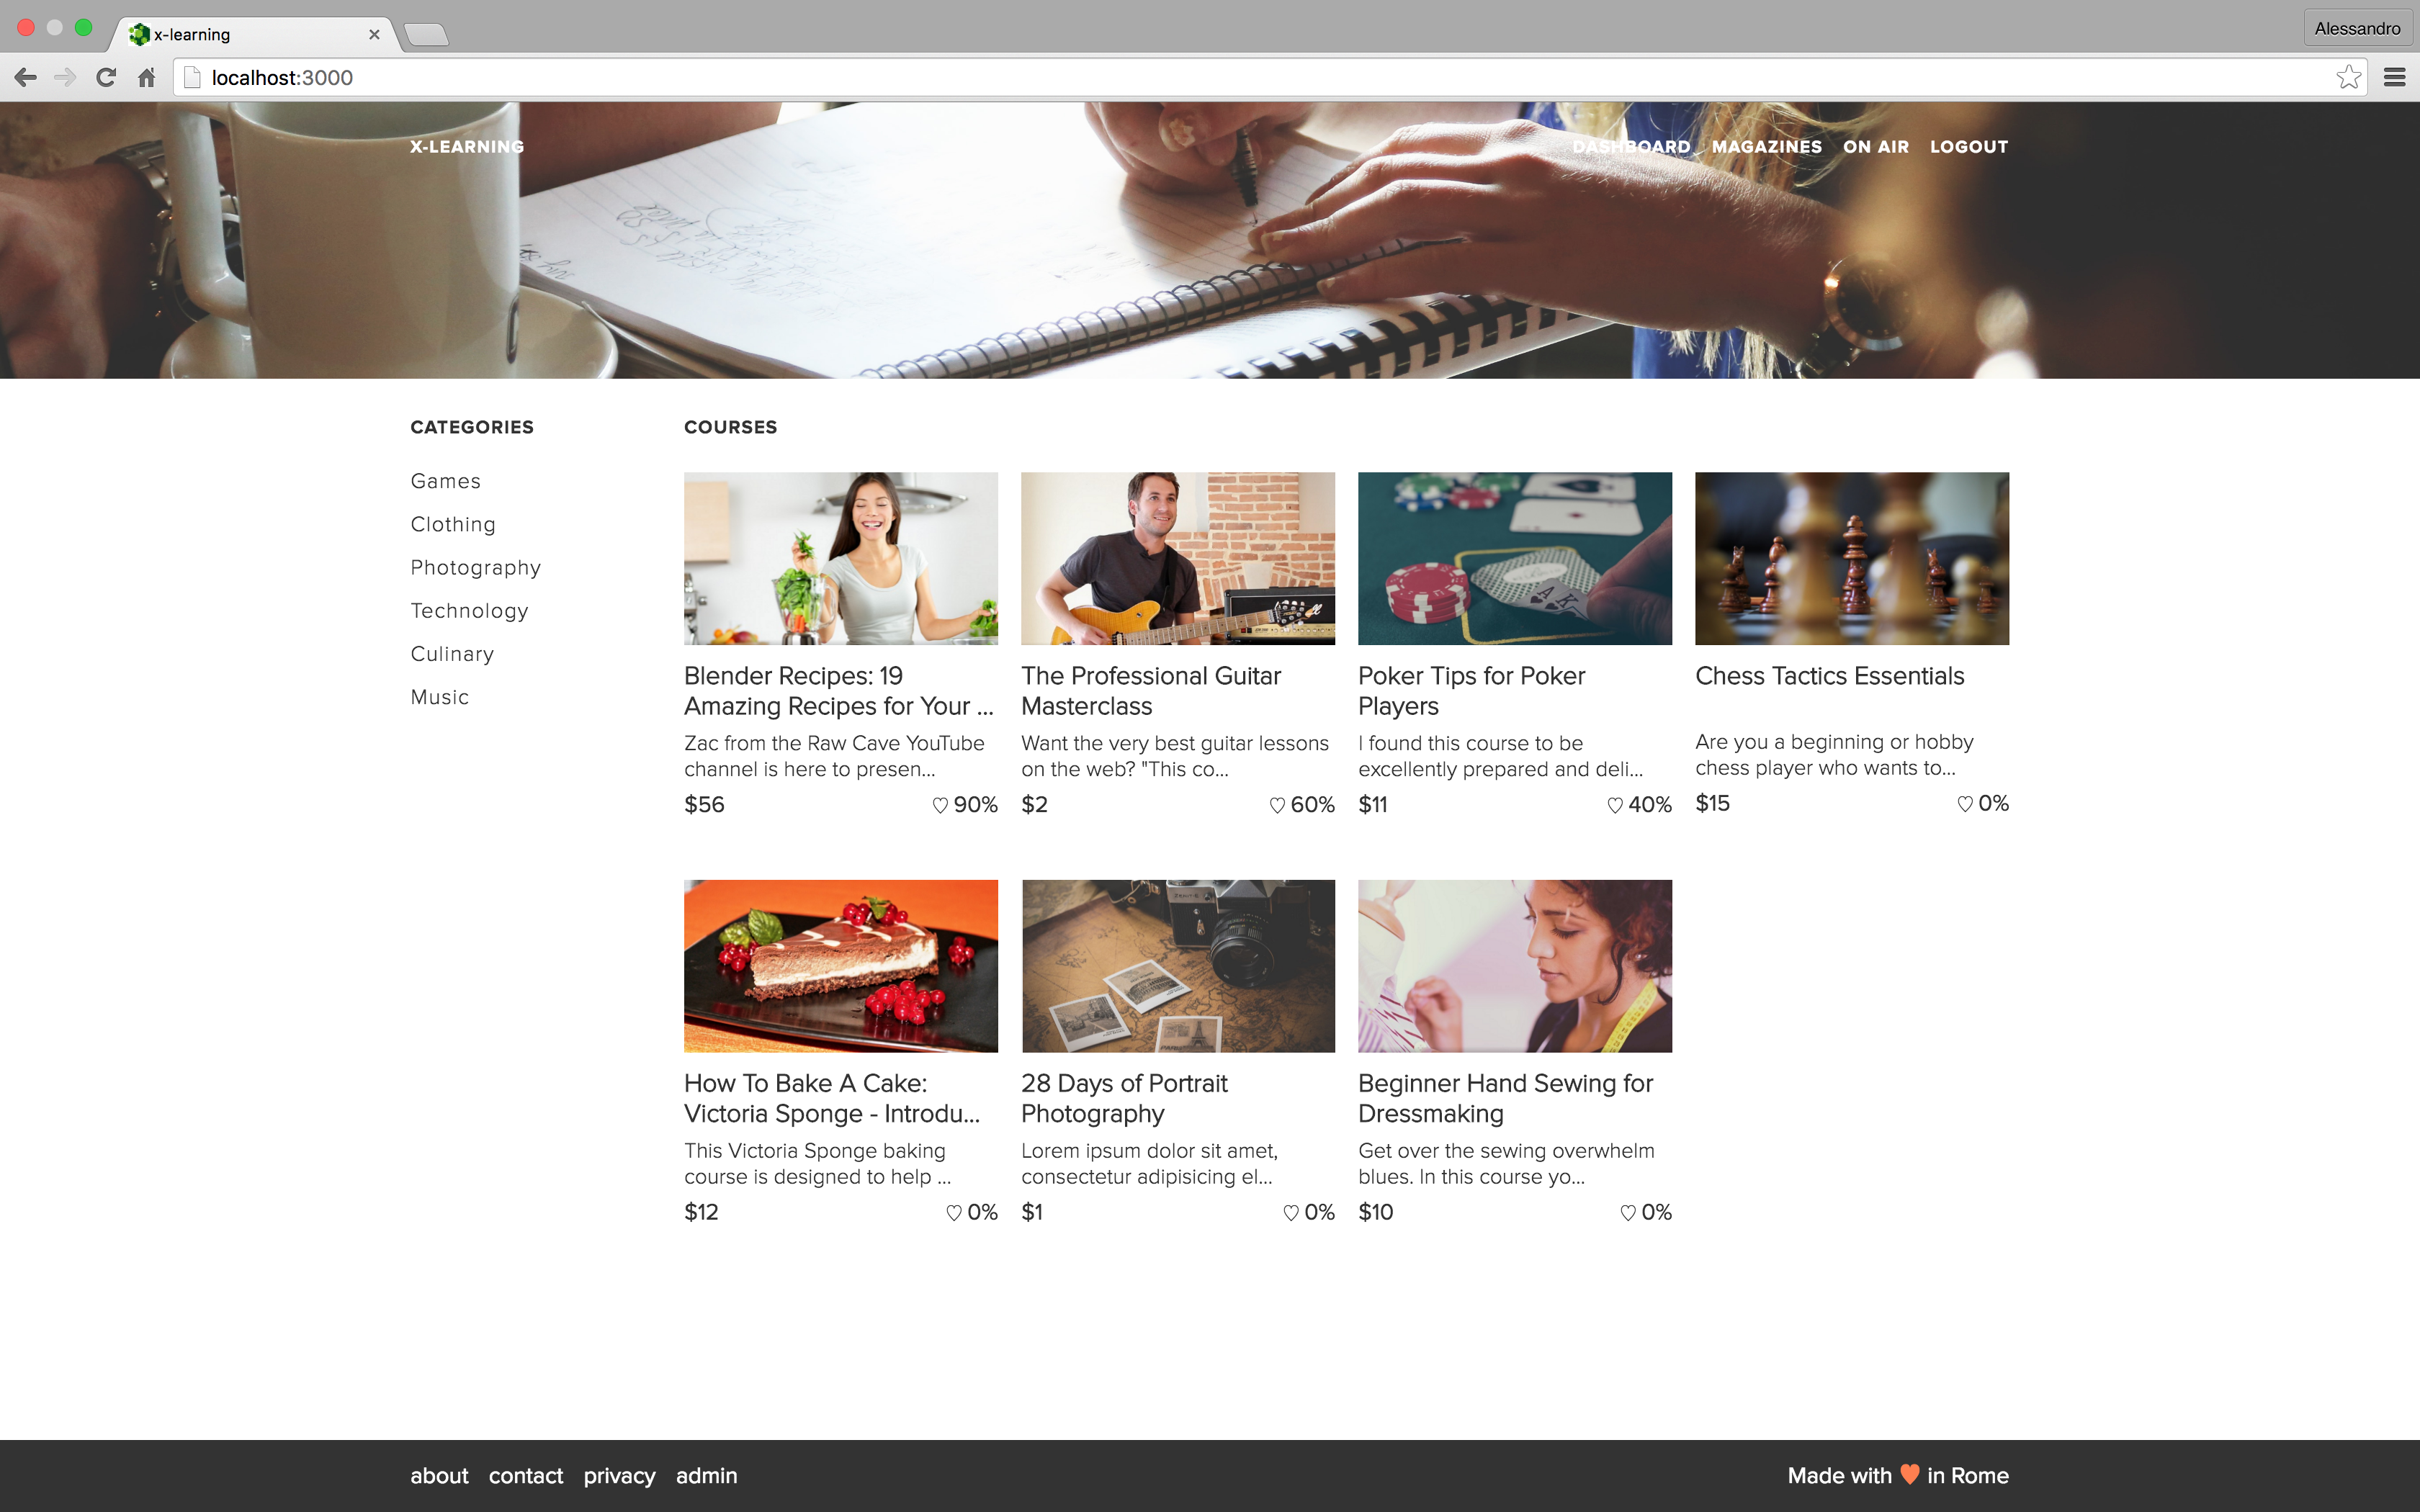
\includegraphics[width=0.9\linewidth]{images/chapter4/page-home.png}
    \captionof{figure}[Page Home]{Page Home}
\end{minipage}


\item \textbf{Page Course} The following image represents the Page Course where all information which composes the course can be found, such as cost, review, video lectures and educational material.
\\
\par

\begin{minipage}{\linewidth}
    \centering
    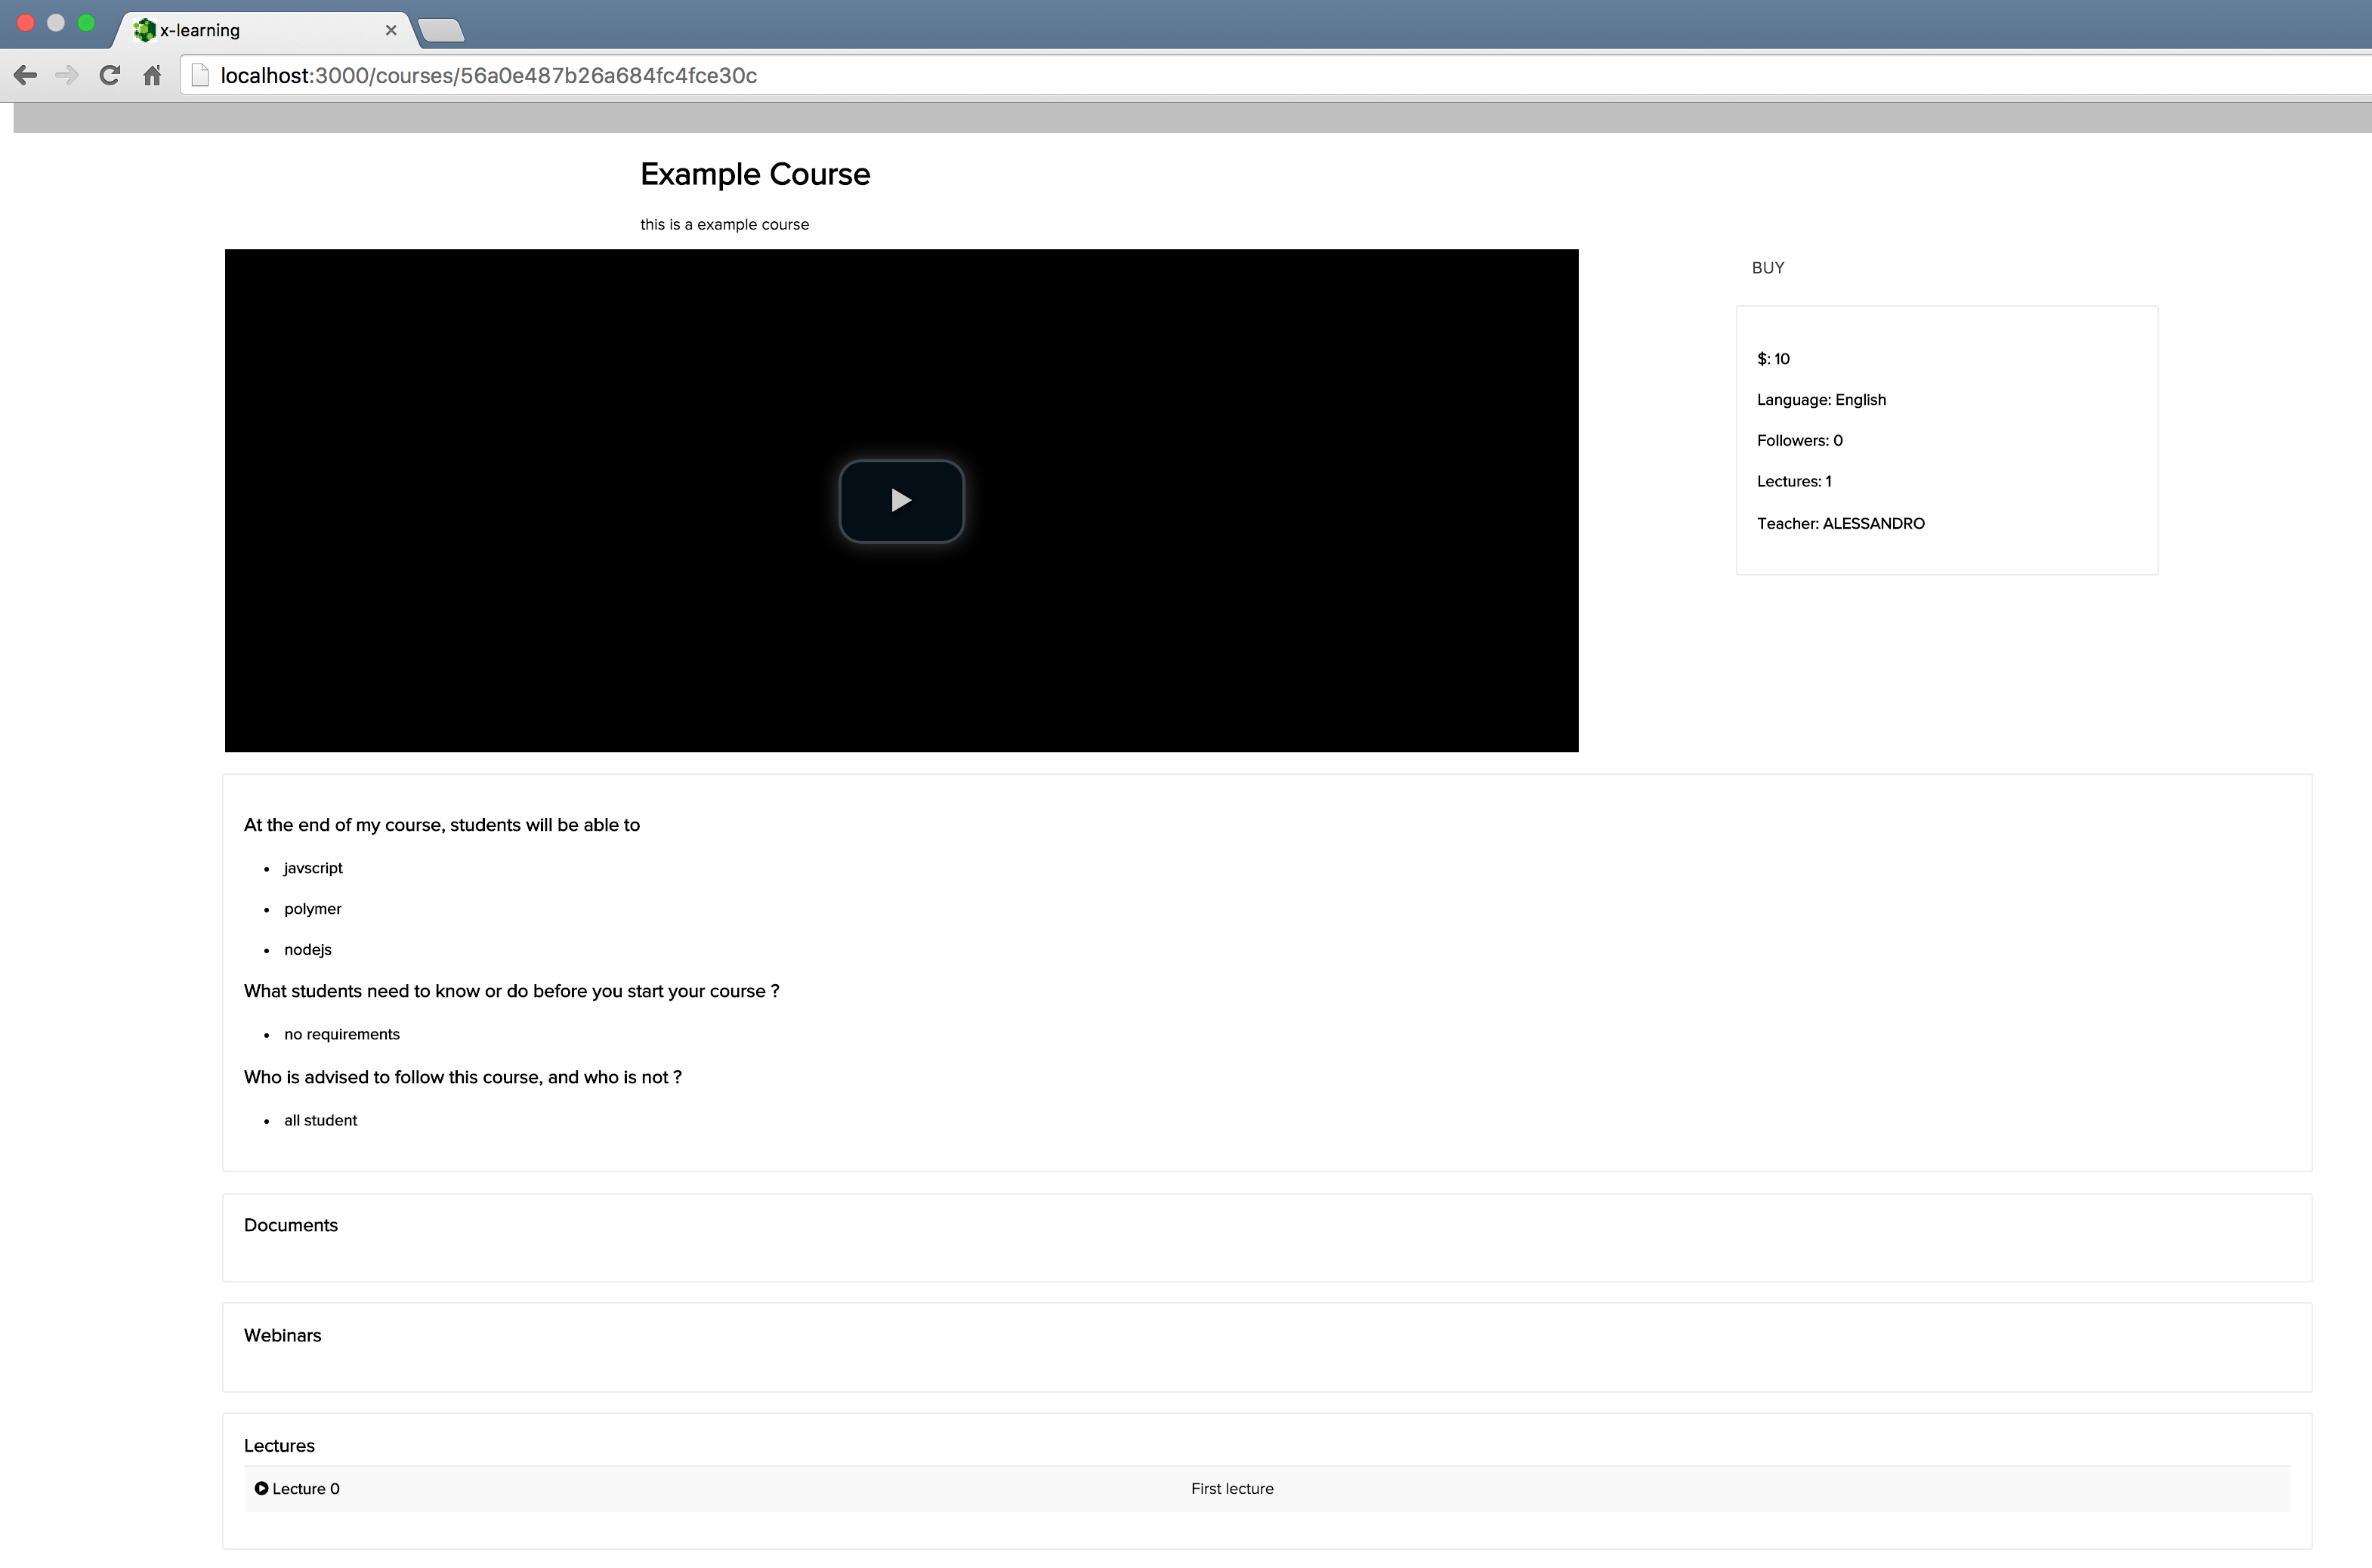
\includegraphics[width=0.9\linewidth]{images/chapter4/page-course.png}
    \captionof{figure}[Page Course]{Page Course}
\end{minipage}


\item \textbf{Page Lecture} The following image represents the page lecture which can allow video lecture visualization.
\\
\par

\begin{minipage}{\linewidth}
    \centering
    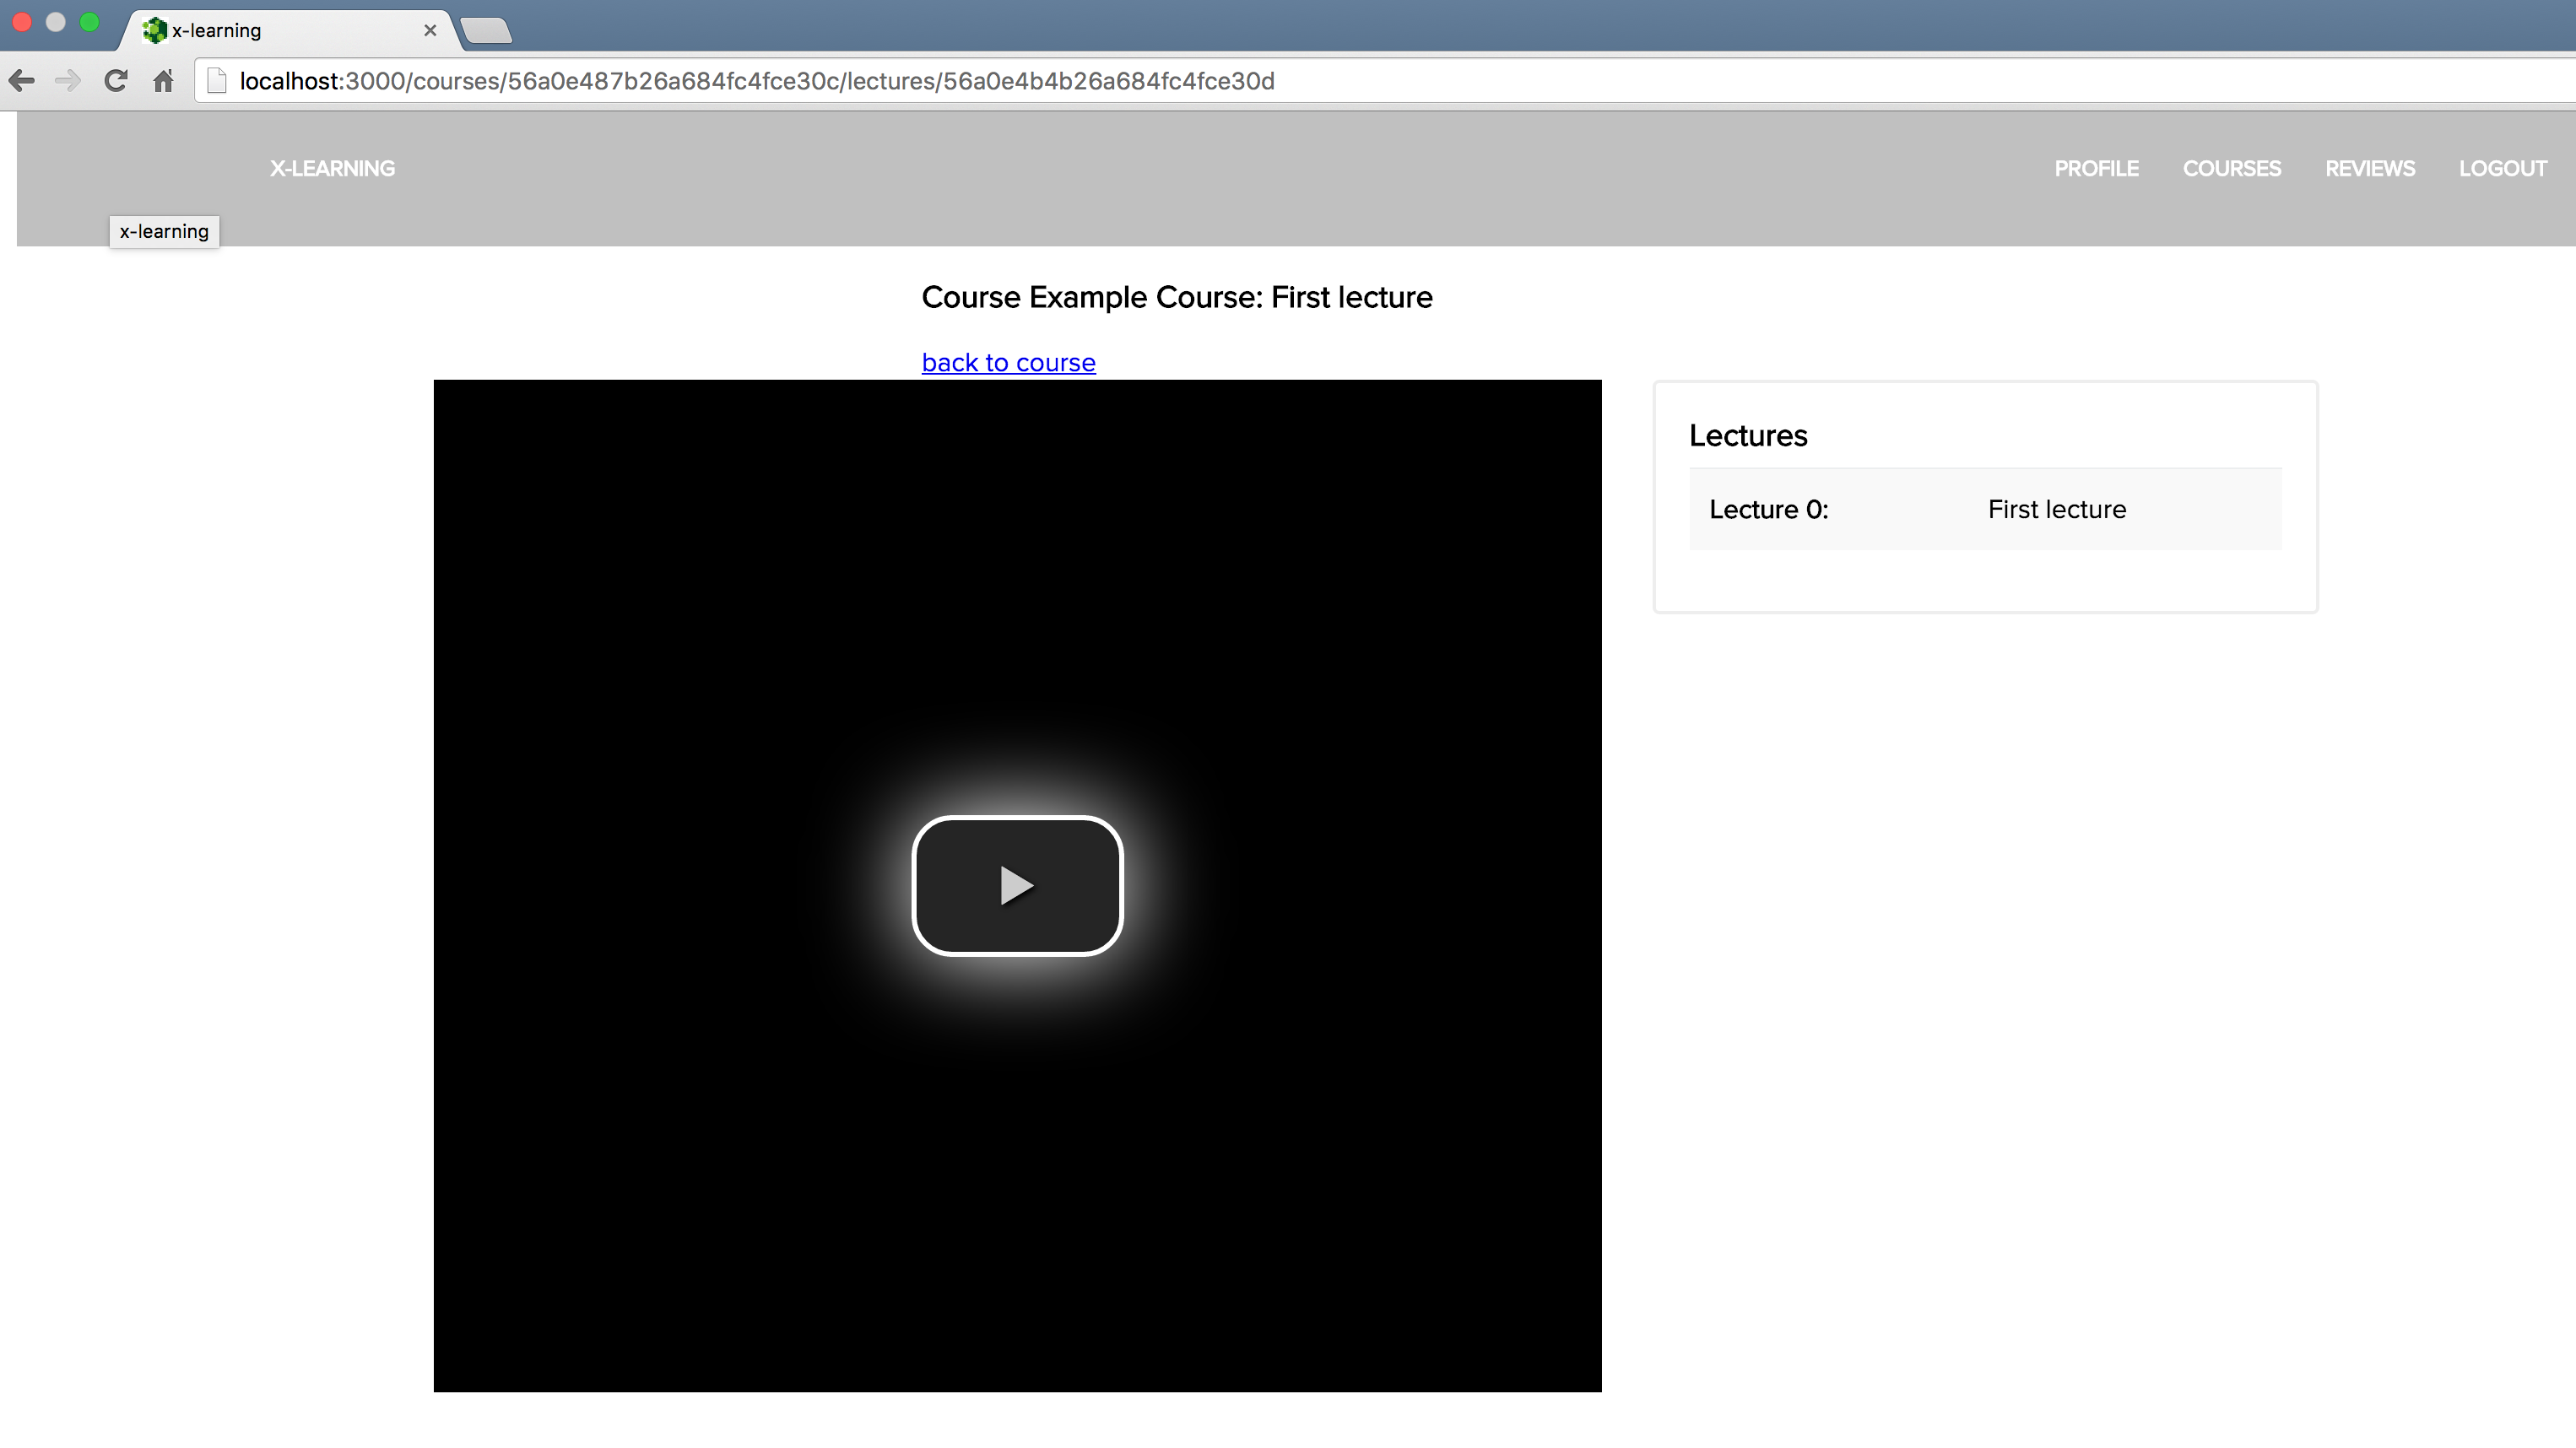
\includegraphics[width=0.9\linewidth]{images/chapter4/page-lecture.png}
    \captionof{figure}[Page Lecture]{Page Lecture}
\end{minipage}


\item \textbf{Page Webinar} The following image represents the Page Webinar which allows to connect to the webinar of a specific course in real time.
\\
\par
\begin{minipage}{\linewidth}
    \centering
    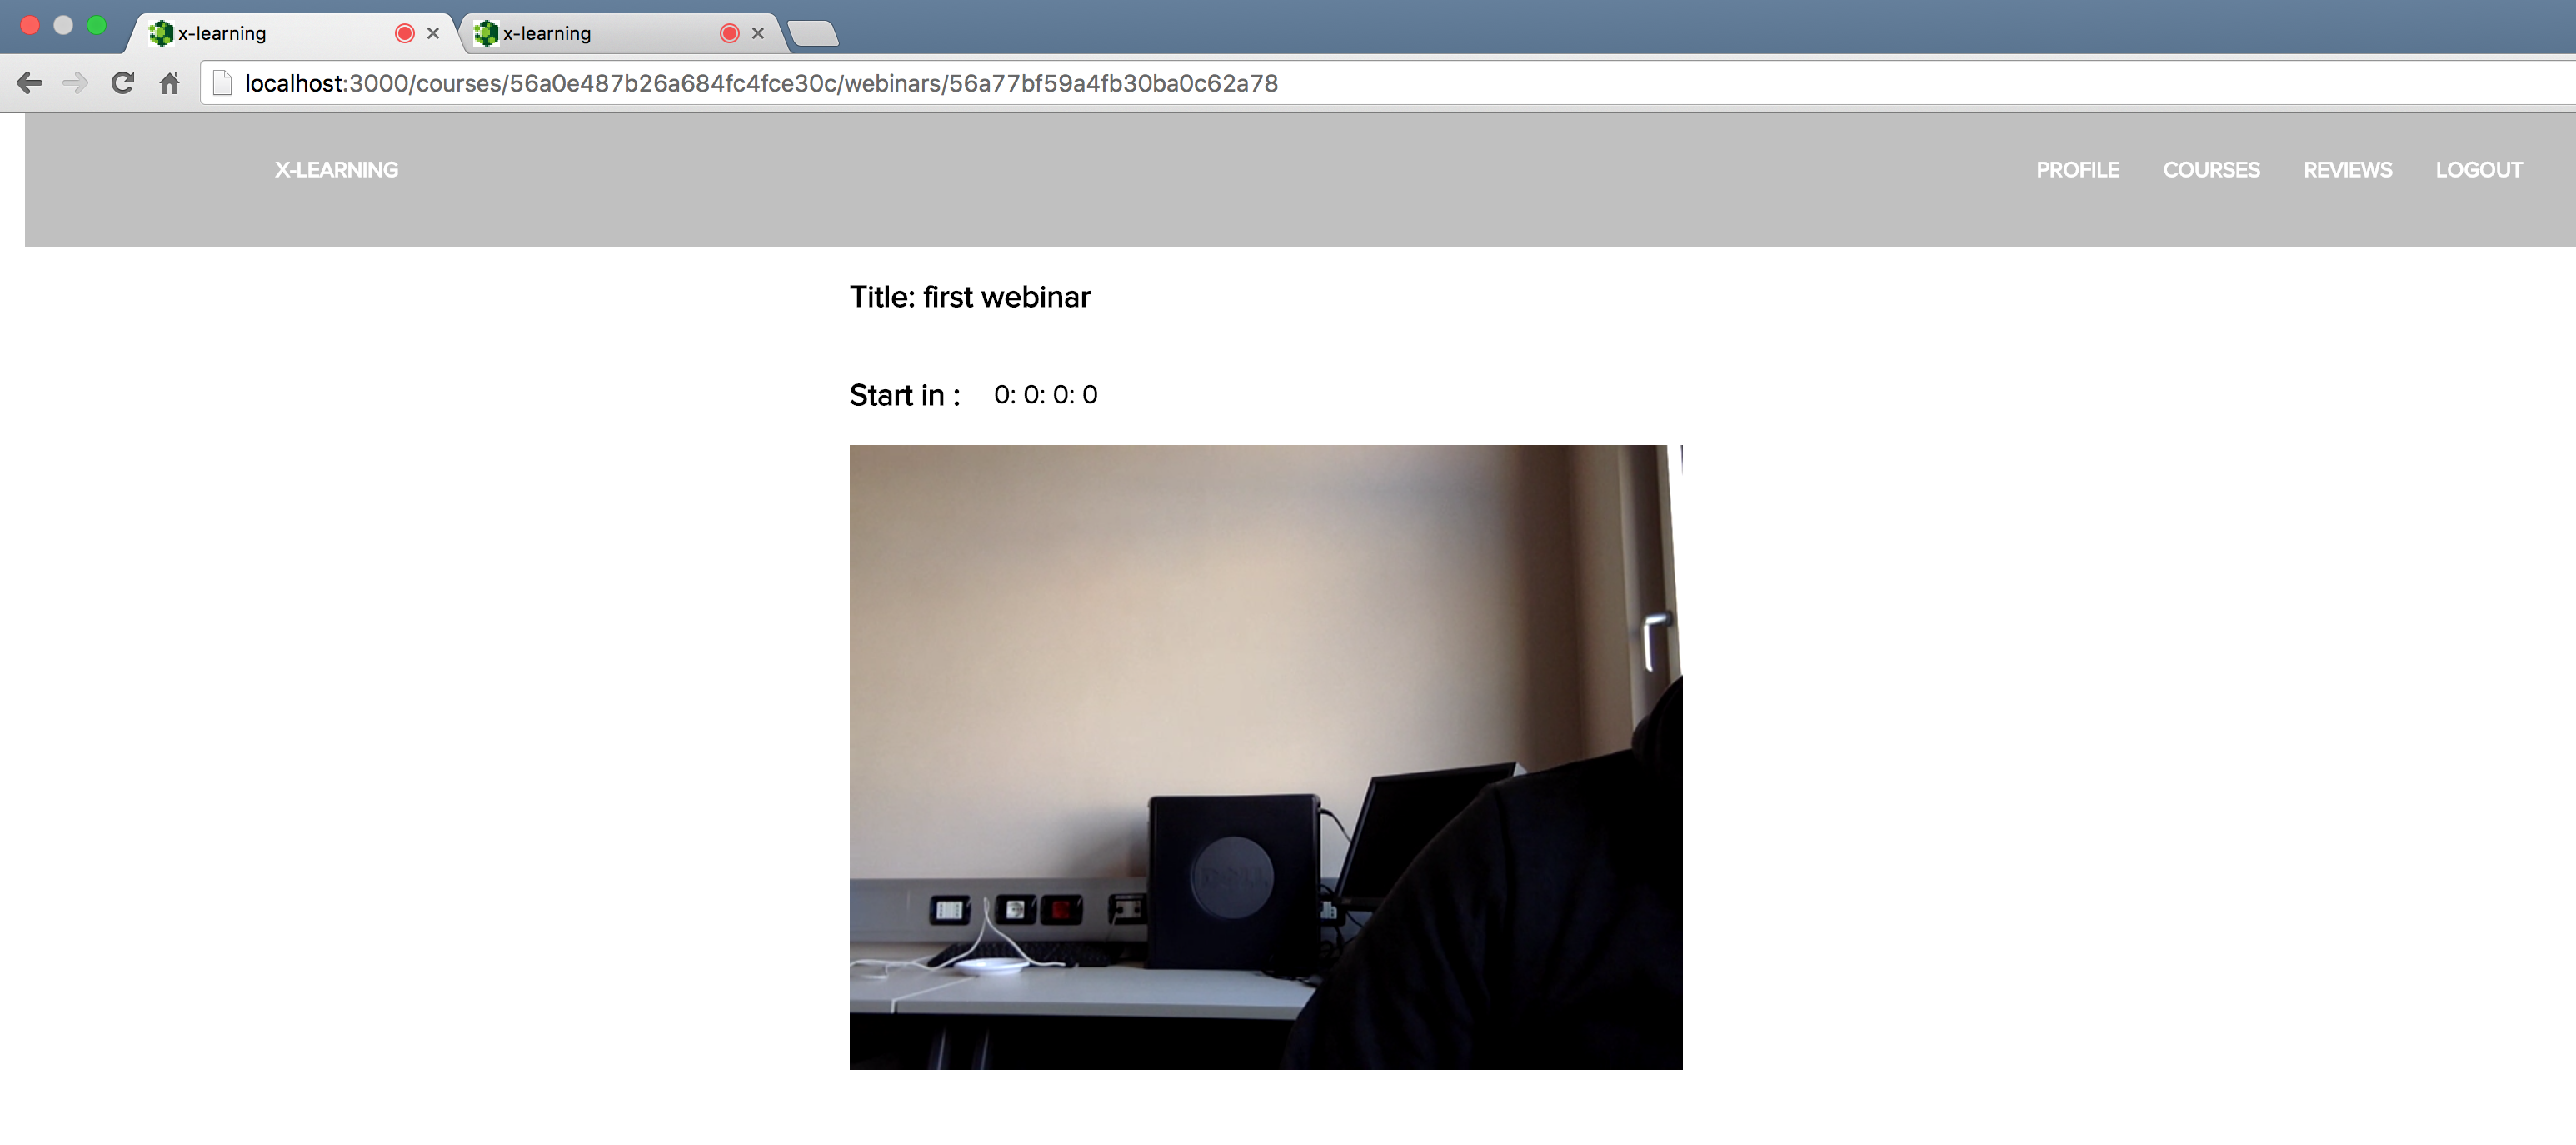
\includegraphics[width=0.9\linewidth]{images/chapter4/page-webinar.png}
    \captionof{figure}[Page Webinar]{Page Webinar}
\end{minipage}

\end{itemize}